% Options for packages loaded elsewhere
\PassOptionsToPackage{unicode}{hyperref}
\PassOptionsToPackage{hyphens}{url}
\documentclass[
  12 pt,
]{article}
\usepackage{xcolor}
\usepackage[margin = 1.0in]{geometry}
\usepackage{amsmath,amssymb}
\setcounter{secnumdepth}{-\maxdimen} % remove section numbering
\usepackage{iftex}
\ifPDFTeX
  \usepackage[T1]{fontenc}
  \usepackage[utf8]{inputenc}
  \usepackage{textcomp} % provide euro and other symbols
\else % if luatex or xetex
  \usepackage{unicode-math} % this also loads fontspec
  \defaultfontfeatures{Scale=MatchLowercase}
  \defaultfontfeatures[\rmfamily]{Ligatures=TeX,Scale=1}
\fi
\usepackage{lmodern}
\ifPDFTeX\else
  % xetex/luatex font selection
\fi
% Use upquote if available, for straight quotes in verbatim environments
\IfFileExists{upquote.sty}{\usepackage{upquote}}{}
\IfFileExists{microtype.sty}{% use microtype if available
  \usepackage[]{microtype}
  \UseMicrotypeSet[protrusion]{basicmath} % disable protrusion for tt fonts
}{}
\makeatletter
\@ifundefined{KOMAClassName}{% if non-KOMA class
  \IfFileExists{parskip.sty}{%
    \usepackage{parskip}
  }{% else
    \setlength{\parindent}{0pt}
    \setlength{\parskip}{6pt plus 2pt minus 1pt}}
}{% if KOMA class
  \KOMAoptions{parskip=half}}
\makeatother
\usepackage{longtable,booktabs,array}
\newcounter{none} % for unnumbered tables
\usepackage{calc} % for calculating minipage widths
% Correct order of tables after \paragraph or \subparagraph
\usepackage{etoolbox}
\makeatletter
\patchcmd\longtable{\par}{\if@noskipsec\mbox{}\fi\par}{}{}
\makeatother
% Allow footnotes in longtable head/foot
\IfFileExists{footnotehyper.sty}{\usepackage{footnotehyper}}{\usepackage{footnote}}
\makesavenoteenv{longtable}
\usepackage{graphicx}
\makeatletter
\newsavebox\pandoc@box
\newcommand*\pandocbounded[1]{% scales image to fit in text height/width
  \sbox\pandoc@box{#1}%
  \Gscale@div\@tempa{\textheight}{\dimexpr\ht\pandoc@box+\dp\pandoc@box\relax}%
  \Gscale@div\@tempb{\linewidth}{\wd\pandoc@box}%
  \ifdim\@tempb\p@<\@tempa\p@\let\@tempa\@tempb\fi% select the smaller of both
  \ifdim\@tempa\p@<\p@\scalebox{\@tempa}{\usebox\pandoc@box}%
  \else\usebox{\pandoc@box}%
  \fi%
}
% Set default figure placement to htbp
\def\fps@figure{htbp}
\makeatother
% definitions for citeproc citations
\NewDocumentCommand\citeproctext{}{}
\NewDocumentCommand\citeproc{mm}{%
  \begingroup\def\citeproctext{#2}\cite{#1}\endgroup}
\makeatletter
 % allow citations to break across lines
 \let\@cite@ofmt\@firstofone
 % avoid brackets around text for \cite:
 \def\@biblabel#1{}
 \def\@cite#1#2{{#1\if@tempswa , #2\fi}}
\makeatother
\newlength{\cslhangindent}
\setlength{\cslhangindent}{1.5em}
\newlength{\csllabelwidth}
\setlength{\csllabelwidth}{3em}
\newenvironment{CSLReferences}[2] % #1 hanging-indent, #2 entry-spacing
 {\begin{list}{}{%
  \setlength{\itemindent}{0pt}
  \setlength{\leftmargin}{0pt}
  \setlength{\parsep}{0pt}
  % turn on hanging indent if param 1 is 1
  \ifodd #1
   \setlength{\leftmargin}{\cslhangindent}
   \setlength{\itemindent}{-1\cslhangindent}
  \fi
  % set entry spacing
  \setlength{\itemsep}{#2\baselineskip}}}
 {\end{list}}
\usepackage{calc}
\newcommand{\CSLBlock}[1]{\hfill\break\parbox[t]{\linewidth}{\strut\ignorespaces#1\strut}}
\newcommand{\CSLLeftMargin}[1]{\parbox[t]{\csllabelwidth}{\strut#1\strut}}
\newcommand{\CSLRightInline}[1]{\parbox[t]{\linewidth - \csllabelwidth}{\strut#1\strut}}
\newcommand{\CSLIndent}[1]{\hspace{\cslhangindent}#1}
\setlength{\emergencystretch}{3em} % prevent overfull lines
\providecommand{\tightlist}{%
  \setlength{\itemsep}{0pt}\setlength{\parskip}{0pt}}
%%%%%%%%%%%%%%%%%%%%%%%%%%%%%%%%%%%%%%%%%%%%%%%%%%%%%%%%%%%%
% Font
%%%%%%%%%%%%%%%%%%%%%%%%%%%%%%%%%%%%%%%%%%%%%%%%%%%%%%%%%%%%

% Set font encoding to T1 (8-bit encoding, 256 glyphs) 
% (improved text handling, especially with non-English
% languages and text containing special characters)
\usepackage[T1]{fontenc}

% Set font to URW Nimbus Roman
% (Times New Roman alternative)
\usepackage{mathptmx}

%%%%%%%%%%%%%%%%%%%%%%%%%%%%%%%%%%%%%%%%%%%%%%%%%%%%%%%%%%%%
% Typsetting
%%%%%%%%%%%%%%%%%%%%%%%%%%%%%%%%%%%%%%%%%%%%%%%%%%%%%%%%%%%%

% Include the package containing commands for page
% orientation
\usepackage{pdflscape}
% Create a new custom command for starting a landscape block
\newcommand{\blandscape}{\begin{landscape}}
% Create a new custom command for ending a landscape block
\newcommand{\elandscape}{\end{landscape}}

% Include package providing fine-tuned typographic
% enhancements
\usepackage{microtype}

% Suppress hyphenation
\usepackage[none]{hyphenat}

% Include package for setting spacing between lines
\usepackage{setspace}
% Set line spacing
\doublespacing

% Indent first paragraph of each section (including
% chapters)
\usepackage{indentfirst}

% Set vertical space between paragraphs
\setlength{\parskip}{1em}

%%%%%%%%%%%%%%%%%%%%%%%%%%%%%%%%%%%%%%%%%%%%%%%%%%%%%%%%%%%%
% Line numbers
%%%%%%%%%%%%%%%%%%%%%%%%%%%%%%%%%%%%%%%%%%%%%%%%%%%%%%%%%%%%

% Include package for line numbering
\usepackage{lineno}
% Set font style and size of line numbers
\renewcommand{\linenumberfont}{\normalfont\tiny}

%%%%%%%%%%%%%%%%%%%%%%%%%%%%%%%%%%%%%%%%%%%%%%%%%%%%%%%%%%%%
% Lists
%%%%%%%%%%%%%%%%%%%%%%%%%%%%%%%%%%%%%%%%%%%%%%%%%%%%%%%%%%%%

% Include package to customise the appearance of itemised
% lists
\usepackage{enumitem}

% Remove extra vertical space that is added above and below
% itemize and enumerate lists
\setlist{nosep}

%%%%%%%%%%%%%%%%%%%%%%%%%%%%%%%%%%%%%%%%%%%%%%%%%%%%%%%%%%%%
% Figures and tables
%%%%%%%%%%%%%%%%%%%%%%%%%%%%%%%%%%%%%%%%%%%%%%%%%%%%%%%%%%%%

% Include package enhancing figure and table placement
% (provides "H" placement specifier forcing the float to
% appear exactly where it is defined)
\usepackage{float}

% Include package used to create tables with cells spanning
% multiple rows
\usepackage{multirow}

%%%%%%%%%%%%%%%%%%%%%%%%%%%%%%%%%%%%%%%%%%%%%%%%%%%%%%%%%%%%
% Captions
%%%%%%%%%%%%%%%%%%%%%%%%%%%%%%%%%%%%%%%%%%%%%%%%%%%%%%%%%%%%

% Define the separator between the label and the caption
% text and make the label bold
\usepackage[labelsep=space, labelfont=bf]{caption}
% Set caption text to be justified
\captionsetup{justification=justified}

%%%%%%%%%%%%%%%%%%%%%%%%%%%%%%%%%%%%%%%%%%%%%%%%%%%%%%%%%%%%
% Uniform Resource Locators (URLs)
%%%%%%%%%%%%%%%%%%%%%%%%%%%%%%%%%%%%%%%%%%%%%%%%%%%%%%%%%%%%

% Include the package to handle URLs
\usepackage{url}

% Redefine the commands that specify where line breaks can
% occur in URLs (\UrlBreaks has a lower penalty, i.e. it is
% more easily chosen, and does not break within a repeating
% sequence)
\renewcommand\UrlBreaks{\do\/\do\:\do\.\do\-}
\renewcommand\UrlBigBreaks{\do\/\do\:\do\.\do\-}

%%%%%%%%%%%%%%%%%%%%%%%%%%%%%%%%%%%%%%%%%%%%%%%%%%%%%%%%%%%%
% Referencing
%%%%%%%%%%%%%%%%%%%%%%%%%%%%%%%%%%%%%%%%%%%%%%%%%%%%%%%%%%%%

% Include the package xr (external references) to allow
% referencing labels from another file
\usepackage{xr}
% Specify the name of the file used for additional
% referencing and define the prefix for the labels
% from the external document
\externaldocument[supp-]{supplementary}

%%%%%%%%%%%%%%%%%%%%%%%%%%%%%%%%%%%%%%%%%%%%%%%%%%%%%%%%%%%%
% Measurement units
%%%%%%%%%%%%%%%%%%%%%%%%%%%%%%%%%%%%%%%%%%%%%%%%%%%%%%%%%%%%

% Include the package that facilitates consistent formatting
% of scientific units and numbers
\usepackage{siunitx}
% Define unit \molar as moles per cubic decimetre
\DeclareSIUnit\molar{\mole\per\cubic\deci\metre}
% Define unit \Molar as small caps "M"
\DeclareSIUnit\Molar{\textsc{m}}
% Define unit \cells as the text "cells"
\DeclareSIUnit\cells{\text{cells}}
% Define unit \litre as lower case "l"
\DeclareSIUnit\litre{l}
% Define unit \vV as v/v
\DeclareSIUnit{\vV}{v/v}
% Define unit \wW as w/w
\DeclareSIUnit{\wW}{w/w}
% Define unit \bp as bp
\DeclareSIUnit{\bp}{bp}
% Define unit \U as U
\DeclareSIUnit{\U}{U}
% Remove the space between the number and the percentage
% sign
\catcode`\%=12\relax
\DeclareSIUnit[number-unit-product = ]\percent{%}
\catcode`\%=14\relax

%%%%%%%%%%%%%%%%%%%%%%%%%%%%%%%%%%%%%%%%%%%%%%%%%%%%%%%%%%%%
% Chemical formulas
%%%%%%%%%%%%%%%%%%%%%%%%%%%%%%%%%%%%%%%%%%%%%%%%%%%%%%%%%%%%

% Include package for typesetting chemical formulas
\usepackage{chemformula}

%%%%%%%%%%%%%%%%%%%%%%%%%%%%%%%%%%%%%%%%%%%%%%%%%%%%%%%%%%%%
% Bookmarks
%%%%%%%%%%%%%%%%%%%%%%%%%%%%%%%%%%%%%%%%%%%%%%%%%%%%%%%%%%%%

% Include package to create hyperlinks, including PDF bookmarks, and
% open all levels of the bookmarks by default
\usepackage[bookmarksopenlevel=\maxdimen]{hyperref}

\usepackage{bookmark}
\IfFileExists{xurl.sty}{\usepackage{xurl}}{} % add URL line breaks if available
\urlstyle{same}
\hypersetup{
  pdftitle={Resident and transient microbial taxa in the gill microbiome of the mussel Mytilus galloprovincialis},
  hidelinks,
  pdfcreator={LaTeX via pandoc}}

\title{\textbf{Resident and transient microbial taxa in the gill microbiome of the mussel \emph{Mytilus galloprovincialis}}}
\author{}
\date{\vspace{-2.5em}}

\begin{document}
\maketitle

%%%%%%%%%%%%%%%%%%%%%%%%%%%%%%%%%%%%%%%%%%%%%%%%%%%%%%%%%%%%
% Captions
%%%%%%%%%%%%%%%%%%%%%%%%%%%%%%%%%%%%%%%%%%%%%%%%%%%%%%%%%%%%

% Set the name for figures to "Figure"
\renewcommand{\figurename}{Fig.}
% Use Arabic numerals to number figures
\renewcommand{\thefigure}{\arabic{figure}}


\vspace{\fill}

Marino Korlević\textsuperscript{1*}, Marsej Markovski\textsuperscript{1}, Damir Kapetanović\textsuperscript{2}, Irena Vardić Smrzlić\textsuperscript{2}, Karla Orlić\textsuperscript{2}, Jakša Bolotin\textsuperscript{3}, Valter Kožul\textsuperscript{3}, Svjetlana Bobanović-Ćolić\textsuperscript{3}, Vedrana Nerlović\textsuperscript{4}, and Lorena Perić\textsuperscript{2*}

\begin{enumerate}
\def\labelenumi{\arabic{enumi}.}
\tightlist
\item
  Centre for Marine Research, Ruđer Bošković Institute, Croatia
\item
  Division for Marine and Environmental Research, Ruđer Bošković Institute, Croatia
\item
  Institute for Marine and Coastal Research, University of Dubrovnik, Croatia
\item
  Faculty of Marine Sciences, University of Split, Croatia
\end{enumerate}

\textsuperscript{*}To whom correspondence should be addressed:\\
Marino Korlević\\
G. Paliaga 5, 52210 Rovinj, Croatia\\
e-mail: \href{mailto:marino.korlevic@irb.hr}{\nolinkurl{marino.korlevic@irb.hr}}\\
ORCID iD: \href{https://orcid.org/0000-0001-5680-3556}{0000-0001-5680-3556}

Lorena Perić\\
Bijenička cesta 54, 10000 Zagreb, Croatia\\
e-mail: \href{mailto:lorena.peric@irb.hr}{\nolinkurl{lorena.peric@irb.hr}}\\
ORCID iD: \href{https://orcid.org/0000-0001-6899-9605}{0000-0001-6899-9605}

% Add line numbers
\linenumbers

% Ensure that numbers are typeset in text mode
\sisetup{mode=text}

% Set the size of indentation to 24 pt
\setlength\parindent{24pt}

% Start a new page
\newpage

\section{Abstract}\label{abstract}

Microorganisms associate with marine bivalves, forming microbial communities collectively known as the bivalve's microbiome. These communities may include resident taxa, associated with the bivalve host throughout its life, and transient taxa, whose presence is temporary and attributed to the passage of, for example, seawater or food through the host. To assess the gill microbiome of the Mediterranean mussel, \emph{Mytilus galloprovincialis} Lamarck, 1819, and its resident and transient taxa, individuals of this important aquaculture species were sampled at two locations on the eastern coast of the Adriatic Sea, Lim Bay and Mali Ston Bay, over one year. The microbiome was characterised using Illumina MiSeq sequencing of the V4 region of the 16S rRNA gene. For comparison, the microbial community in the surrounding seawater and sediment was also assessed at the same time and locations. The structure of the gill microbiome, determined at the OTU level, was distinct from the microbial community in both the surrounding seawater and sediment and did not differ between the two locations. However, it showed differences between months, indicating temporal dynamics. Taxonomic analysis revealed the presence of both resident and transient microbial taxa in the gill microbiome. Members without known relatives within \emph{Endozoicomonadaceae} (i.e.~unclassified \emph{Endozoicomonadaceae}) were present in the gills of mussels from both locations and throughout the study period and appeared to be resident members. In contrast, \emph{Endozoicomonas} and ``\emph{Candidatus} Endoecteinascidia'' were transient, appearing in the gill microbiome of mussels from both locations only in certain months, as were \emph{Vibrio} and members without known relatives within \emph{Vibrionaceae} (i.e.~unclassified \emph{Vibrionaceae}), with the distinction that these were specific to Lim Bay. Overall, the results of this study show that the gill microbiome of the mussel \emph{Mytilus galloprovincialis} differs from the microbial community in the surrounding seawater and sediment, exhibits temporal dynamics, and contains both resident and transient microbial taxa.

\noindent
\textbf{Keywords:} gill microbiome, Mediterranean mussel, \emph{Mytilus galloprovincialis}, aquaculture, Adriatic Sea, 16S rRNA gene sequencing, temporal changes, \emph{Gammaproteobacteria}
\newpage

\section{Introduction}\label{introduction}

Marine animals, including bivalves, are associated with various microorganisms such as archaea, bacteria, viruses, protists, and fungi {[}\citeproc{ref-Apprill2017}{1}, \citeproc{ref-Salloum2025}{2}{]}. These microbes, collectively known as the animal's microbiome, can reside on or within the animal's body {[}\citeproc{ref-Apprill2017}{1}, \citeproc{ref-Petersen2018}{3}{]}. If located inside the body, they may live either outside or within host cells. Notably, microbes within host cells can inhabit specialised cells dedicated to housing symbionts, forming a particularly intimate type of symbiosis {[}\citeproc{ref-Petersen2018}{3}{]}. The close relationship between the host and its microbiome can be viewed as a holobiont: an integrated community in which the animal and its symbiotic microbes support each other {[}\citeproc{ref-Salloum2025}{2}, \citeproc{ref-Margulis1991}{4}{]}. Furthermore, as suggested by the hologenome concept, the genetic content of the host and the microbes in its microbiome should be considered a single evolutionary unit, meaning that host evolution is influenced by its microbiome {[}\citeproc{ref-Salloum2025}{2}, \citeproc{ref-Bordenstein2015}{5}{]}.

Studies on bivalves, such as mussels, oysters, clams, and cockles, have shown that the bivalve's microbiome may include both resident members, associated with the host throughout its life, and transient members, whose presence is temporary and attributed, for example, to the passage of seawater or food through the animal {[}\citeproc{ref-Munoz-Martinez2026}{6}, \citeproc{ref-Pierce2018}{7}{]}. Evidence from oysters suggests that most microbes in the bivalve's microbiome are resident members {[}\citeproc{ref-Unzueta-Martinez2022a}{8}{]}. Additionally, as previously reported for oysters, these microbes may be acquired by the host vertically, transmitted from parent to offspring, horizontally, adopted from the surrounding environment, or through a combination of these processes {[}\citeproc{ref-Petersen2018}{3}, \citeproc{ref-Bright2010}{9}, \citeproc{ref-Unzueta-Martinez2022}{10}{]}. Studies have also shown that the microbiome of various bivalves, such as mussels, oysters, clams, and cockles, differs from the microbial community in surrounding seawater or sediment, highlighting the resident nature of most microbiome members {[}\citeproc{ref-Munoz-Martinez2026}{6}, \citeproc{ref-Unzueta-Martinez2022}{10}--\citeproc{ref-Vezzulli2018}{16}{]}. In addition to differing from the surrounding environment, the microbiome of different bivalve species also varies between body parts, such as the gut, gills, and haemolymph {[}\citeproc{ref-Unzueta-Martinez2022}{10}, \citeproc{ref-Lokmer2016}{13}, \citeproc{ref-Musella2020}{14}, \citeproc{ref-Vezzulli2018}{16}, \citeproc{ref-Dube2019}{17}{]}, and is, to some extent and for certain body parts, specific to the host species {[}\citeproc{ref-Munoz-Martinez2026}{6}, \citeproc{ref-Akter2023}{11}, \citeproc{ref-Pierce2019}{15}, \citeproc{ref-Vezzulli2018}{16}, \citeproc{ref-Gignoux-Wolfsohn2024}{18}{]}. Although most microbes in the bivalve's microbiome appear to be resident members, a portion remains transient {[}\citeproc{ref-Unzueta-Martinez2022a}{8}{]}, as suggested by studies of mussels and oysters reporting temporal changes {[}\citeproc{ref-Akter2023}{11}, \citeproc{ref-Pierce2019}{15}, \citeproc{ref-Nguyen2020}{19}, \citeproc{ref-Pierce2016}{20}{]}. The bivalve's microbiome can also differ between geographic locations {[}\citeproc{ref-Unzueta-Martinez2022a}{8}, \citeproc{ref-Gignoux-Wolfsohn2024}{18}, \citeproc{ref-Nguyen2020}{19}, \citeproc{ref-delRio-Lavin2023}{21}, \citeproc{ref-Lokmer2016a}{22}{]}, indicating that local conditions may also have an influence. Interestingly, the microbiome of mussels transported from one geographic location to another converges towards that of native bivalves, highlighting the importance of local conditions {[}\citeproc{ref-Peruzzo2026}{23}, \citeproc{ref-Sun2025}{24}{]}.

Microbes forming the bivalve's microbiome belong to various high-rank bacterial taxa, including the \emph{Pseudomonadota} classes \emph{Alphaproteobacteria} and \emph{Gammaproteobacteria}, \emph{Bacillota}, \emph{Bacteroidota}, \emph{Fusobacteriota}, and \emph{Spirochaetota} {[}\citeproc{ref-Munoz-Martinez2026}{6}, \citeproc{ref-Gignoux-Wolfsohn2024}{18}, \citeproc{ref-Lasa2019}{25}{]}. Members of these taxa have also been found in the microbiome of the Mediterranean mussel, \emph{Mytilus galloprovincialis} Lamarck, 1819 {[}\citeproc{ref-Munoz-Martinez2026}{6}, \citeproc{ref-Akter2023}{11}, \citeproc{ref-Musella2020}{14}, \citeproc{ref-Vezzulli2018}{16}, \citeproc{ref-delRio-Lavin2023}{21}, \citeproc{ref-Peruzzo2026}{23}, \citeproc{ref-Auguste2024a}{26}--\citeproc{ref-Zardinoni2024}{31}{]}, an important aquaculture bivalve species widely distributed across the Mediterranean Sea, including the Adriatic Sea {[}\citeproc{ref-Gosling2003b}{32}--\citeproc{ref-Wenne2022}{36}{]}. Studies focusing on \emph{M. galloprovincialis} have reported patterns of dynamics for this species' microbiome similar to those previously mentioned for the bivalve's microbiome in general. Specifically, differences between the microbiome and the ambient seawater have been reported {[}\citeproc{ref-Akter2023}{11}, \citeproc{ref-Musella2020}{14}, \citeproc{ref-Vezzulli2018}{16}, \citeproc{ref-Palladino2023}{28}, \citeproc{ref-Zardinoni2024}{31}{]}, as well as microbiome specificity for this host species {[}\citeproc{ref-Munoz-Martinez2026}{6}, \citeproc{ref-Akter2023}{11}, \citeproc{ref-Vezzulli2018}{16}{]} and its variation between body parts {[}\citeproc{ref-Musella2020}{14}, \citeproc{ref-Vezzulli2018}{16}{]}, sampling periods {[}\citeproc{ref-Akter2023}{11}, \citeproc{ref-Peruzzo2026}{23}, \citeproc{ref-Palladino2023}{28}, \citeproc{ref-Wathsala2021}{30}{]}, and geographic locations {[}\citeproc{ref-delRio-Lavin2023}{21}, \citeproc{ref-Peruzzo2026}{23}, \citeproc{ref-Palladino2023}{28}{]}.

In general, studies assessing the bivalve's microbiome have focused on gut tissue {[}\citeproc{ref-Salloum2025}{2}{]}. Similarly, research on the \emph{M. galloprovincialis} microbiome has usually examined the gut microbiome {[}\citeproc{ref-Akter2023}{11}, \citeproc{ref-Vezzulli2018}{16}, \citeproc{ref-delRio-Lavin2023}{21}, \citeproc{ref-Palladino2023}{28}, \citeproc{ref-Wathsala2021}{30}{]} or assessed the microbiome of the whole individual without a tissue-specific sampling approach {[}\citeproc{ref-Munoz-Martinez2026}{6}, \citeproc{ref-Peruzzo2026}{23}, \citeproc{ref-Bozcal2020}{27}, \citeproc{ref-Schoinas2023}{29}{]}. Consequently, a limited number of studies have described the temporal and spatial dynamics of the microbiome in other body parts, such as gills and haemolymph {[}\citeproc{ref-Sun2025}{24}, \citeproc{ref-Auguste2024a}{26}, \citeproc{ref-Zardinoni2024}{31}{]}. As the mussel \emph{M. galloprovincialis} is a filter-feeding animal {[}\citeproc{ref-Gosling2003a}{37}{]}, its gills form a uniquely complex interface between the host and the surrounding environment, are in constant contact with seawater, and may be influenced by sediment resuspension {[}\citeproc{ref-Rosa2018}{38}, \citeproc{ref-Ward2004}{39}{]}. Therefore, this study focused on assessing the gill microbiome of individuals of this bivalve species, as well as the microbial community in the surrounding seawater and sediment, from two important and geographically distant bivalve aquaculture locations on the eastern coast of the Adriatic Sea, namely Lim Bay and Mali Ston Bay {[}\citeproc{ref-BratosCetinic2024}{40}{]}, over a period of one year. The study locations are in two legally protected marine reserve areas with distinct hydrological conditions and productivity, typical of the Adriatic Sea biogeographical regions to which they belong {[}\citeproc{ref-Bosak2013}{41}--\citeproc{ref-Skejic2015}{44}{]}. More precisely, the aims of this study were to: (i) compare the mussel gill microbiome with the microbial community in the surrounding seawater and sediment, (ii) determine differences in the gill microbiome between the two aquaculture locations, and (iii) assess changes in the gill microbiome during the one-year study period. Unlike earlier work, this study uses multiple biological replicates to capture inter-individual variation in the gill microbiome, as this tissue is a dynamic barrier that continually interacts with its environment.
\newpage

\section{Methods}\label{methods}

\subsection{Sampling}\label{sampling}

This study was conducted at two bivalve aquaculture locations: Lim Bay in the north and Mali Ston Bay in the south of the eastern Adriatic Sea coast (Fig. \ref{fig:map}). Mussels of the species \emph{M. galloprovincialis}, seawater, and sediment were sampled in July, September, and November 2020 and January, March, and May 2021 (Supplementary Tables \ref{supp-tab:nseq-notus-seawater-sediment} and \ref{supp-tab:nseq-notus-gills}), as described in Žurga et al. {[}\citeproc{ref-Zurga2024}{45}{]} and Orlić et al. {[}\citeproc{ref-Orlic2025a}{46}{]}. Briefly, locally produced adult mussels were deployed at an aquaculture site at a depth of 10 \unit{\m} in Lim Bay (\ang{45;7;50}N, \ang{13;41;20}E) and 6 \unit{\m} in Mali Ston Bay (\ang{42;52;16}N, \ang{17;42;12}E), following common farming practices at these locations (Fig. \ref{fig:map}). Bottom depths in Lim Bay and Mali Ston Bay were 28 and 8 \unit{\m}, respectively. At each sampling date, 10 individuals were collected, their gills excised, and snap-frozen in liquid nitrogen. Seawater was collected at a depth close to that at which mussels were deployed, specifically 8 \unit{\m} in Lim Bay and 5 \unit{\m} in Mali Ston Bay, using a Niskin bottle and filtered (0.35--1 \unit{\l}) through 0.2 \unit{\um} membrane filters. Filters were transferred into 2 \unit{\ml} cryotubes and snap-frozen in liquid nitrogen. As this is the initial study conducted in these coastal areas of the eastern Adriatic Sea, sediment samples were also analysed to establish a baseline characterisation of sediment microbial communities associated with bivalve farming environments. Sediment was also sampled because mussels constantly filter large volumes of seawater through their gills, and the seawater they filter may contain sediment particles resuspended by continuous seafloor disturbance caused by currents and waves {[}\citeproc{ref-Rosa2018}{38}, \citeproc{ref-Ward2004}{39}, \citeproc{ref-Asmus2011}{47}, \citeproc{ref-Velasco2005}{48}{]}. Surface sediment exposed to and disturbed by the movement of water masses was collected using an Ekman grab sampler, transferred into 2 \unit{\ml} cryotubes, and snap-frozen in liquid nitrogen. Upon arrival at the laboratory, samples of gills and sediment, as well as membrane filters, were stored at \qty{-80}{\degreeCelsius} until further processing. To provide a broader environmental context, seawater and sediment were sampled not only at the aquaculture site but also at a nearby site where no mussel-growing structures were present and which was sufficiently close to minimise spatial variability in baseline seawater and sediment characteristics. This additional site in both Lim Bay (\ang{45;7;57}N, \ang{13;38;27}E) and Mali Ston Bay (\ang{42;51;59}N, \ang{17;42;5}E; Fig. \ref{fig:map}) was designated as the control site. Seawater at this site was sampled at the same depth as at the aquaculture site. Seawater abiotic parameters (temperature, salinity, dissolved oxygen, and chlorophyll \emph{a}) displayed seasonal patterns typical of the eastern Adriatic Sea {[}\citeproc{ref-Zurga2024}{45}{]}. Sediment was classified as slightly gravelly mud at the aquaculture site and slightly gravelly sandy mud at the control site in Lim Bay, and as gravelly mud at the aquaculture site and gravelly muddy sand at the control site in Mali Ston Bay (unpublished data).

\begin{figure}[t]

{\centering 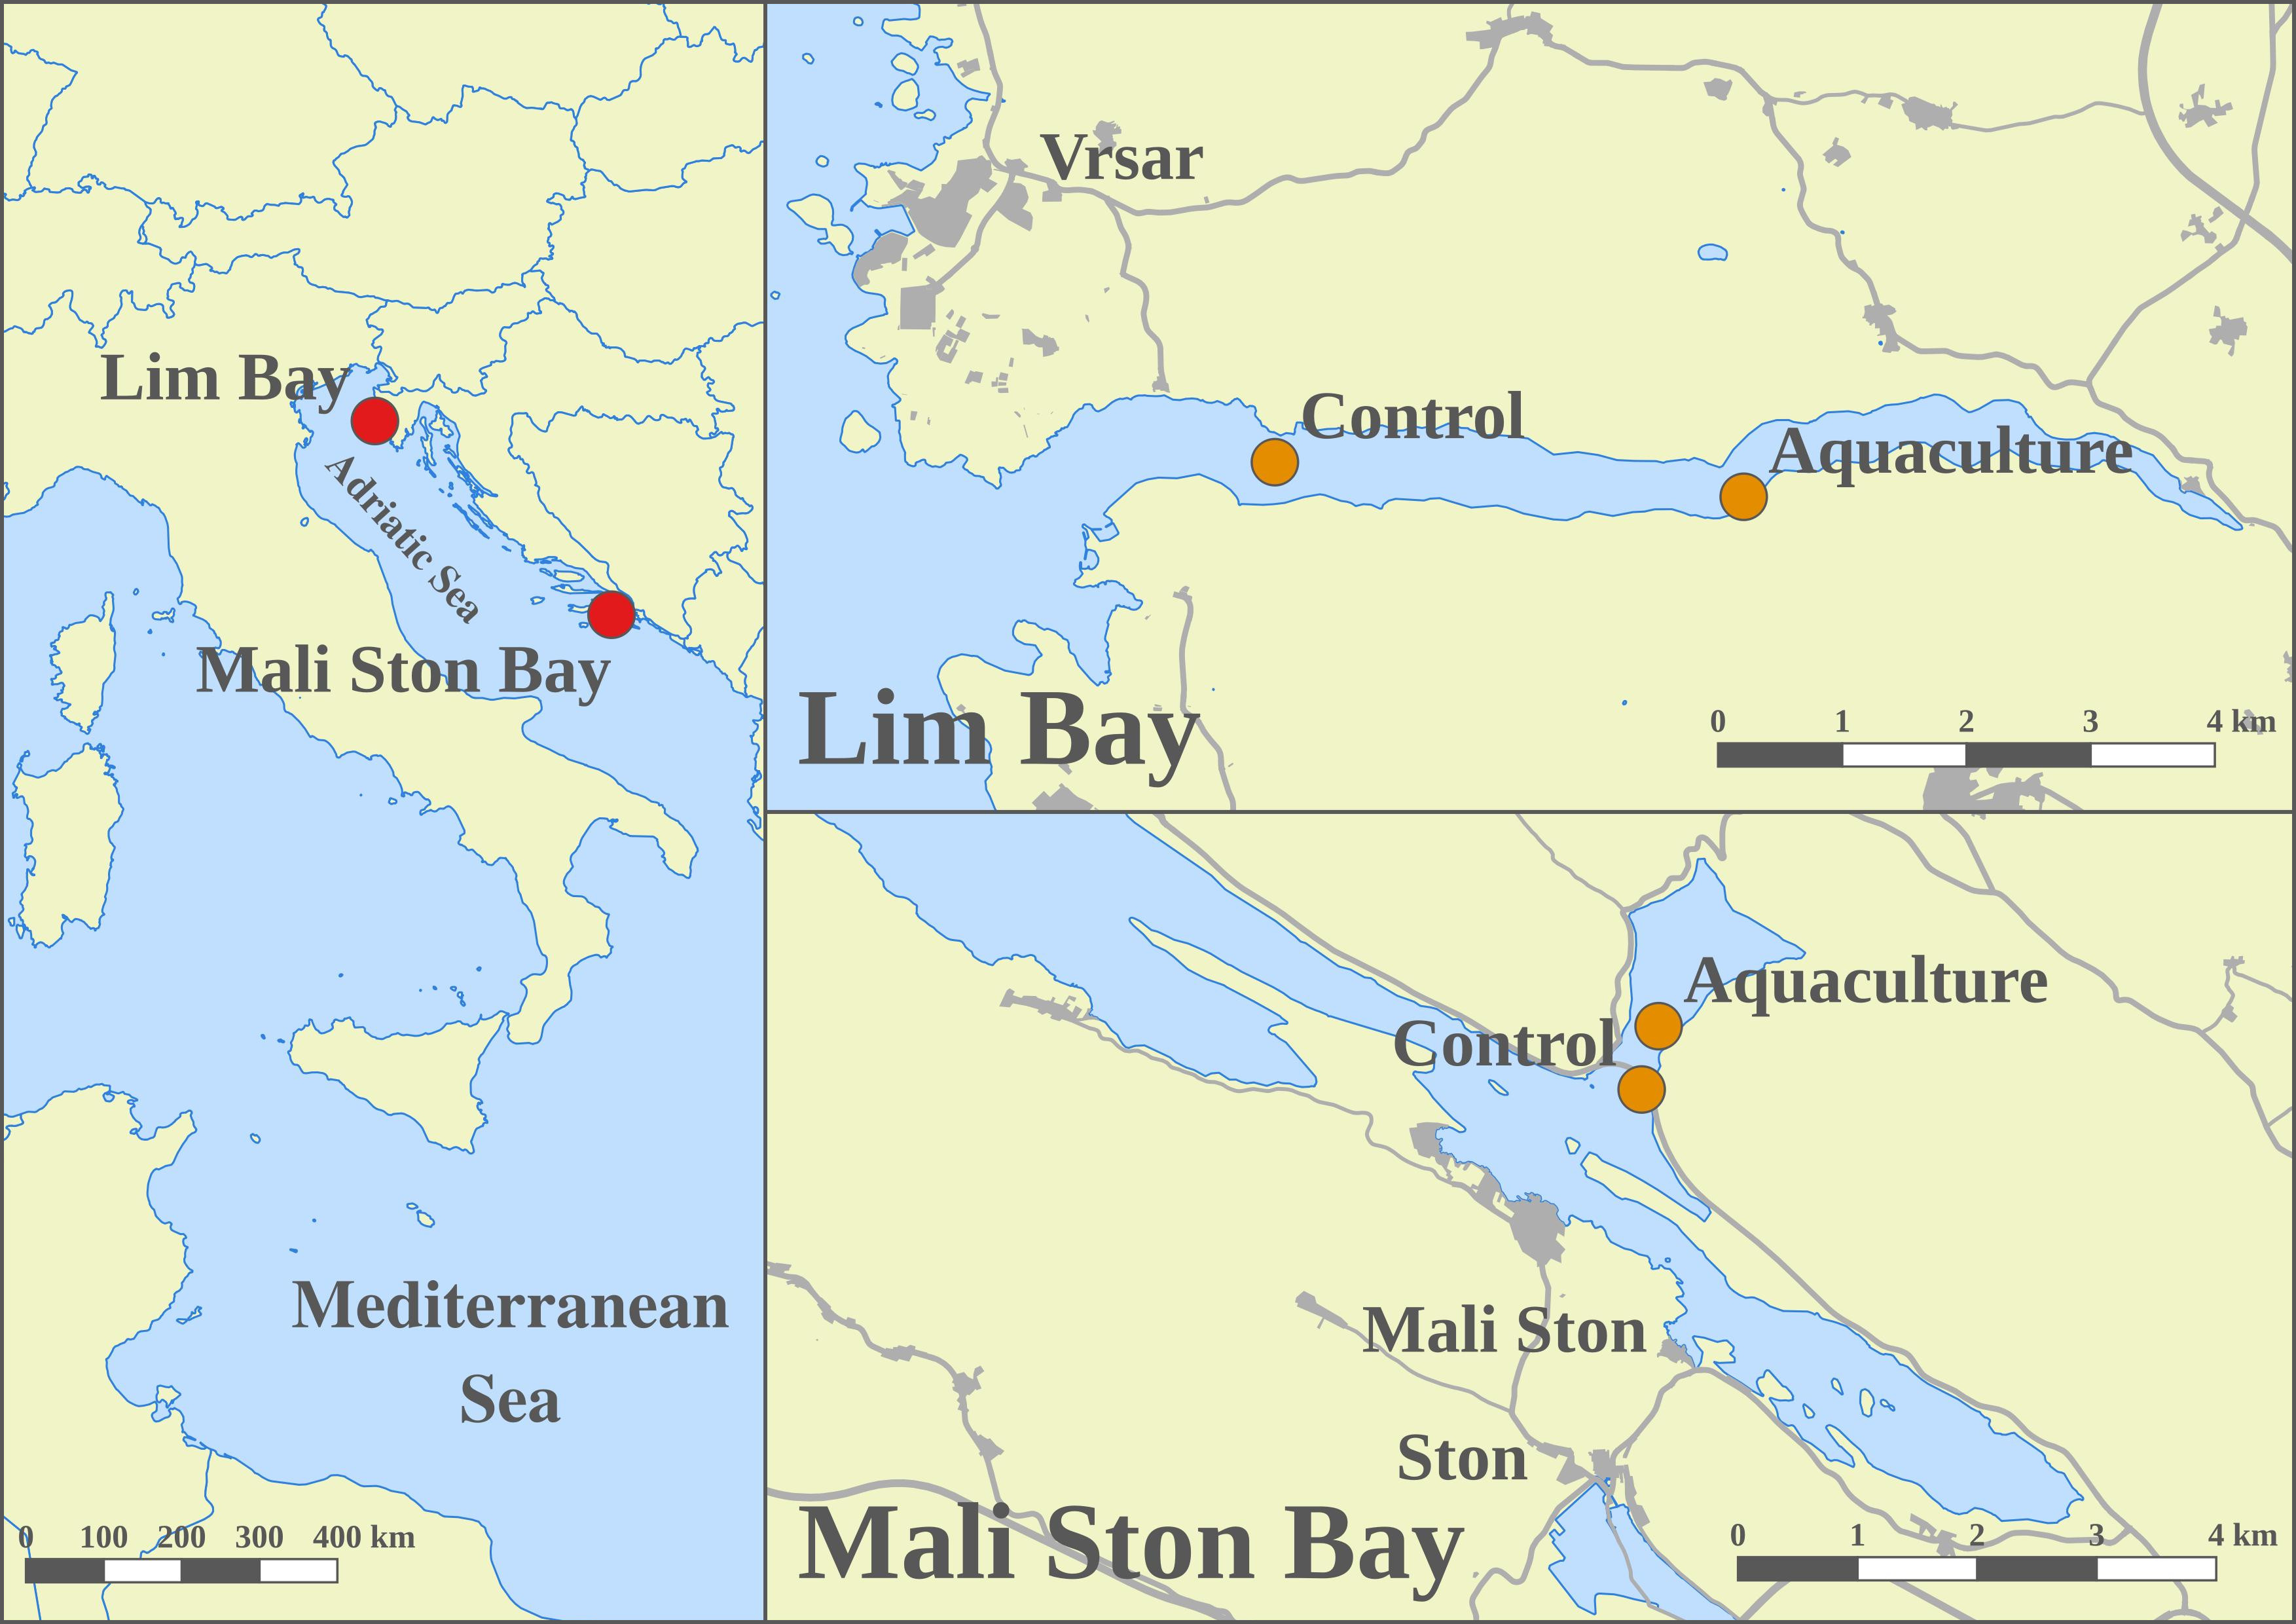
\includegraphics[width=1\linewidth]{../results/figures/map} 

}

\caption{Sampling locations and sites in the Adriatic Sea. At each location, namely Lim Bay and Mali Ston Bay, samples were collected from one aquaculture site and one control site (© OpenStreetMap contributors, \url{https://www.openstreetmap.org/copyright})}\label{fig:map}
\end{figure}



\subsection{DNA isolation}\label{dna-isolation}

Total DNA from gills (32--123 \unit{\mg} of snap-frozen tissue) and 0.2 \unit{\um} membrane filters was isolated according to Massana et al. {[}\citeproc{ref-Massana1997}{49}{]} with slight modifications. After extraction with organic solvents, 1/10 volume of 3 \unit{\Molar} sodium acetate (pH 5.2) was added. DNA was precipitated by adding 1 volume of cold (\qty{-20}{\degreeCelsius}) isopropanol and incubating the mixture for 1 \unit{\hour} or overnight at \qty{-20}{\degreeCelsius}. The pellet obtained after centrifugation at 20,000 × \emph{g} and \qty{4}{\degreeCelsius} for 20 \unit{\minute} was washed twice with 500 \unit{\ul} of cold (\qty{-20}{\degreeCelsius}) 70\unit{\percent} ethanol. After each wash, the pellet was centrifuged at 20,000 × \emph{g} and \qty{4}{\degreeCelsius} for 5 \unit{\minute}. Air-dried pellets were resuspended in 100 \unit{\ul} of deionised water for DNA isolated from gills and 50 \unit{\ul} for DNA isolated from membrane filters. Total DNA from sediment was isolated as described in Markovski et al. {[}\citeproc{ref-Markovski2022}{50}{]}. This is a modified protocol {[}\citeproc{ref-Pjevac2018}{51}{]} of the isolation procedure described in Zhou et al. {[}\citeproc{ref-Zhou1996}{52}{]}. Briefly, 2 \unit{\gram} of sediment was mixed with extraction buffer and proteinase K, and incubated by horizontal shaking at 37 \unit{\degreeCelsius} for 30 \unit{\minute}. After SDS was added, the mixture was incubated again by horizontal shaking at 65 \unit{\degreeCelsius} for 60 \unit{\minute}. Sediment particles were removed by centrifugation and the supernatant was extracted three times with an equal volume of chloroform:isoamyl alcohol (1:1). DNA was precipitated by adding isopropanol and incubating the mixture at 22 \unit{\degreeCelsius} for 60 \unit{\minute}. The pellet obtained by centrifugation was washed twice with cold (\qty{-20}{\degreeCelsius}) 70\unit{\percent} ethanol, air-dried, and resuspended in 100 \unit{\ul} of deionised water. DNA isolated from gills, membrane filters, and sediment was treated with RNase A at a final concentration of 200 \unit{\ug\per\ml} at 37 \unit{\degreeCelsius} for 2 \unit{\hour}. DNA concentration was determined using the Quant-iT PicoGreen dsDNA Assay Kit (Invitrogen, USA) according to the manufacturer's instructions. DNA from gills was diluted to 10 \unit{\ng\per\ul}, and DNA from membrane filters and sediment to 1 \unit{\ng\per\ul}.

\subsection{Illumina 16S rRNA sequencing}\label{illumina-16s-rrna-sequencing}

The V4 region of the 16S rRNA gene was amplified using a two-step PCR procedure. In the first PCR, 515F (Parada; 5\('\)-GTGYCAGCMGCCGCGGTAA-3\('\)) and 806R (Apprill; 5\('\)-GGACTACNVGGGTWTCTAAT-3\('\)) primers from the Earth Microbiome Project (\url{https://earthmicrobiome.org/protocols-and-standards/16s}) were used {[}\citeproc{ref-Apprill2015}{53}--\citeproc{ref-Parada2016}{56}{]}, each with a sequence tag at the 5\('\) end. Four parallel PCRs were performed to amplify the target region from each DNA sample. Each 25 \unit{\ul} reaction contained 1 × Q5 Reaction Buffer, 0.2 \unit{\milli\Molar} dNTP mix, 0.7 \unit{\mg\per\ml} bovine serum albumin (BSA), 0.5 \unit{\micro\Molar} forward and
reverse primers, 0.5 \unit{\U} Q5 High-Fidelity DNA Polymerase (New England Biolabs, USA), and 50 \unit{\ng} DNA template from gills or 5 \unit{\ng} from membrane filters and sediment. The cycling conditions were: initial denaturation at 98 \unit{\degreeCelsius} for 30 \unit{\s}; 25 cycles of denaturation at 98 \unit{\degreeCelsius} for 10 \unit{\s}, annealing at 50 \unit{\degreeCelsius} for 30 \unit{\s}, and elongation at 72 \unit{\degreeCelsius} for 5 \unit{\s} for reactions with DNA from gills or 30 \unit{\s} for reactions with DNA from membrane filters and sediment. PCR cycling ended with a final elongation at 72 \unit{\degreeCelsius} for 2 \unit{\minute}. The higher amount of DNA template (50 \unit{\ng}) and shorter elongation time (5 \unit{\s}) used for amplifying the target region from DNA isolated from gills were optimised to reduce amplification of non-specific fragments. The four parallel reactions were pooled, and PCR products were purified using the GeneJET PCR Purification Kit (Thermo Fisher Scientific, USA) according to the manufacturer's instructions. The protocol without isopropanol addition was followed to avoid co-purification of primer-dimers. The column was eluted in 30 \unit{\ul} deionised water.

Purified PCR products were sent to IMGM Laboratories, Martinsried, Germany, for Illumina MiSeq sequencing (2 × 250 \unit{\bp}). Before sequencing, the second PCR in the two-step PCR procedure was performed using primers that bind to the sequence tag added during the first PCR. In addition to the gill, seawater, and sediment samples, two positive and two negative controls were sequenced. Each positive control consisted of four parallel PCRs using genomic DNA from a mock community composed of evenly mixed DNA from 20 bacterial strains (ATCC MSA-1002, ATCC, USA) as the DNA template. Each negative control comprised four parallel PCRs without a DNA template. One positive and one negative control were processed according to the PCR procedure for gill samples, and one positive and one negative control according to the PCR procedure for seawater and sediment samples.

\subsection{Sequence and data analysis}\label{sequence-and-data-analysis}

Sequences obtained were analysed using mothur (version 1.48.2) {[}\citeproc{ref-Schloss2009}{57}{]} following the MiSeq Standard Operating Procedure (MiSeq SOP; \url{https://mothur.org/wiki/miseq_sop}) {[}\citeproc{ref-Kozich2013}{58}{]} and recommendations from the Riffomonas project to enhance data reproducibility (\url{https://riffomonas.org}). For alignment and classification, the SILVA SSU Ref NR 99 database (release 138.2; \url{https://www.arb-silva.de}) was used {[}\citeproc{ref-Quast2013}{59}, \citeproc{ref-Yilmaz2014}{60}{]}. Sequences were clustered into operational taxonomic units (OTUs) using a 97\unit{\percent} similarity threshold. In this study, sequences that could not be classified into any taxon were labelled ``No Relative'', whereas sequences that could not be classified to any known taxon within a specific taxonomic group are referred to as members without known relatives within that group.

Data processing and visualisation were performed using R (version 4.6.1) {[}\citeproc{ref-R-base}{61}{]} with the packages vegan (version 2.7-5) {[}\citeproc{ref-R-vegan}{62}{]} and tidyverse (version 2.0.0) {[}\citeproc{ref-R-tidyverse}{63}, \citeproc{ref-tidyverse2019}{64}{]}, as well as several other packages {[}\citeproc{ref-R-bookdown}{65}--\citeproc{ref-tinytex2019}{88}{]}. Mean values of the observed number of OTUs, Chao1, abundance-based coverage estimator (ACE), exponential of the Shannon diversity index, and Inverse Simpson diversity index were calculated from 100 subsamples of OTU abundances (rarefaction) to account for differences in sequencing depth {[}\citeproc{ref-Schloss2024}{89}{]}. Each subsample was obtained by randomly selecting, without replacement, a number of sequences equal to the minimum number of sequences per sample using vegan's function \texttt{rrarefy} {[}\citeproc{ref-R-vegan}{62}{]}. The richness estimators Chao1 and ACE were obtained using vegan's function \texttt{estimateR}, while the Shannon and Inverse Simpson diversity indices were calculated using vegan's function \texttt{diversity} {[}\citeproc{ref-R-vegan}{62}{]}. To express both diversity indices as the effective number of OTUs, the exponential of the Shannon diversity index was calculated {[}\citeproc{ref-Jost2006}{90}{]}. Non-metric multidimensional scaling (NMDS) was performed on Bray--Curtis dissimilarities using vegan's function \texttt{metaMDS} {[}\citeproc{ref-R-vegan}{62}, \citeproc{ref-Borcard2018}{91}, \citeproc{ref-Legendre2012}{92}{]}. To account for differences in sequencing depth, Bray--Curtis dissimilarities were calculated using vegan's function \texttt{avgdist} by randomly subsampling OTU abundances to the minimum number of sequences per sample 100 times and calculating mean Bray--Curtis dissimilarities across all subsamples (rarefaction) {[}\citeproc{ref-R-vegan}{62}, \citeproc{ref-Schloss2024}{89}{]}. Differences between communities from distinct environments, sites, locations, and months were tested by performing permutational multivariate analysis of variance (PERMANOVA) on the same Bray--Curtis dissimilarities using vegan's function \texttt{adonis2} with 999 permutations, followed by pairwise PERMANOVA comparisons using pairwiseAdonis's function \texttt{pairwise.adonis}, also with 999 permutations, when more than two groups of samples were tested (Bonferroni correction was applied to address the multiple comparisons problem) {[}\citeproc{ref-R-vegan}{62}, \citeproc{ref-R-pairwiseAdonis}{76}{]}. Multivariate homogeneity of group dispersions was assessed using vegan's function \texttt{betadisper} and tested using vegan's function \texttt{permutest} with 999 permutations {[}\citeproc{ref-R-vegan}{62}{]}. Significant PERMANOVA results accompanied by significant differences in the homogeneity of group dispersions (\emph{p} \textless{} 0.05) were taken into account when group sizes were balanced or, in one case, reported separately {[}\citeproc{ref-Anderson2013}{93}{]}. Differences between richness estimators, diversity indices, and proportions of taxa were tested using the Mann--Whitney \emph{U} test with the function \texttt{wilcox.test} when two groups were compared, or the Kruskal--Wallis \emph{H} test with the function \texttt{kruskal.test}, followed by pairwise comparisons with the Mann--Whitney \emph{U} test using the function \texttt{pairwise.wilcox.test}, when more than two groups were compared {[}\citeproc{ref-R-base}{61}{]}. The Bonferroni correction was applied to address the multiple comparisons problem.

From six sampling months, two locations (Lim Bay and Mali Ston Bay), and two sites (aquaculture and control), 24 seawater and 24 sediment samples were processed. Additionally, from 10 individuals collected at the aquaculture site during the same months and locations, 120 gill samples were processed. This resulted in a total of 168 samples, of which 149 yielded sufficient sequences for further analysis (Supplementary Tables \ref{supp-tab:nseq-notus-seawater-sediment} and \ref{supp-tab:nseq-notus-gills}). From these samples, a total of 2.1 million sequences were obtained after quality curation and exclusion of sequences without known relatives (no relative sequences), as well as eukaryotic, chloroplast, and mitochondrial sequences. The number of sequences per sample ranged from 2,062 to 60,611 (Supplementary Tables \ref{supp-tab:nseq-notus-seawater-sediment} and \ref{supp-tab:nseq-notus-gills}). These sequences were clustered into a total of 66,695 different OTUs. For seawater and sediment samples, as well as for gill samples with a high number of OTUs, the rarefaction curves did not level off, even with the highest sequencing effort, as is commonly observed in high-throughput 16S rRNA amplicon sequencing approaches (Supplementary Figs. \ref{supp-fig:rarefaction-a} and \ref{supp-fig:rarefaction-b}). However, for gill samples with a low number of OTUs, the rarefaction curves did level off. The absence of levelling off in the rarefaction curves for seawater, sediment, and some gill samples suggests that increasing sequencing depth could reveal additional OTUs. Based on the positive controls (mock community ATCC MSA-1002), a sequencing error rate of 0.04\unit{\percent} was calculated, which is comparable to previously reported values for next-generation 16S rRNA amplicon sequencing {[}\citeproc{ref-Markovski2022}{50}, \citeproc{ref-Kozich2013}{58}, \citeproc{ref-Korlevic2021a}{94}, \citeproc{ref-Schloss2016}{95}{]}. In addition, all 20 strains whose DNA was present in the mock community were detected. The two negative controls processed with the samples yielded 10 and 12 sequences after sequence quality curation.
\newpage

\section{Results}\label{results}

To assess the richness and diversity of microbial communities, the observed number of OTUs, the richness estimators Chao1 and ACE, the exponential of the Shannon diversity index, and the Inverse Simpson diversity index were calculated at the OTU level for the sampled environments (seawater, sediment, and the gills of \emph{M. galloprovincialis}) at both aquaculture and control sites (Fig. \ref{fig:alpha}). Statistically significant changes were found for all parameters (Kruskal--Wallis \emph{H} test, all \emph{p} \textless{} 0.0001; Supplementary Table \ref{supp-tab:kruskal-wallis}). The sediment microbial community had the highest observed number of OTUs (aquaculture, 928.9--1,343.4 OTUs; control, 1,049.7--1,448.1 OTUs), followed by the seawater community (aquaculture, 188.4--423.8 OTUs; control, 216.7--455.9 OTUs), and the gill microbiome (aquaculture, 39.8--746.9 OTUs). No significant differences in the observed number of OTUs were found between the aquaculture and control sites for the sediment and seawater communities (Fig. \ref{fig:alpha} and Supplementary Table \ref{supp-tab:kruskal-wallis}). The same pattern was observed for the exponential of the Shannon diversity index and the Inverse Simpson diversity index. However, when the richness estimators Chao1 and ACE were calculated, differences between the gill microbiome and seawater microbial communities at the aquaculture and control sites were no longer observed (Fig. \ref{fig:alpha} and Supplementary Table \ref{supp-tab:kruskal-wallis}). Additionally, location-specific changes for all sampled environments, as well as temporal changes for the gill microbiome, were evaluated. Neither parameter showed differences between the sampling locations, except for the Inverse Simpson diversity index of sediment communities, which showed higher values in Mali Ston Bay (175.3--803.1 OTUs) than in Lim Bay (106.4--289.6 OTUs; Mann--Whitney \emph{U} test, \emph{p} \textless{} 0.01). Furthermore, for the gill microbiome, only the richness estimators Chao1 and ACE showed differences across sampling months (Kruskal--Wallis \emph{H} test, both \emph{p} \textless{} 0.05). However, comparisons between sampling months using the pairwise Mann--Whitney \emph{U} test showed no significant differences (Bonferroni-corrected).

\begin{figure}[ht!]

{\centering 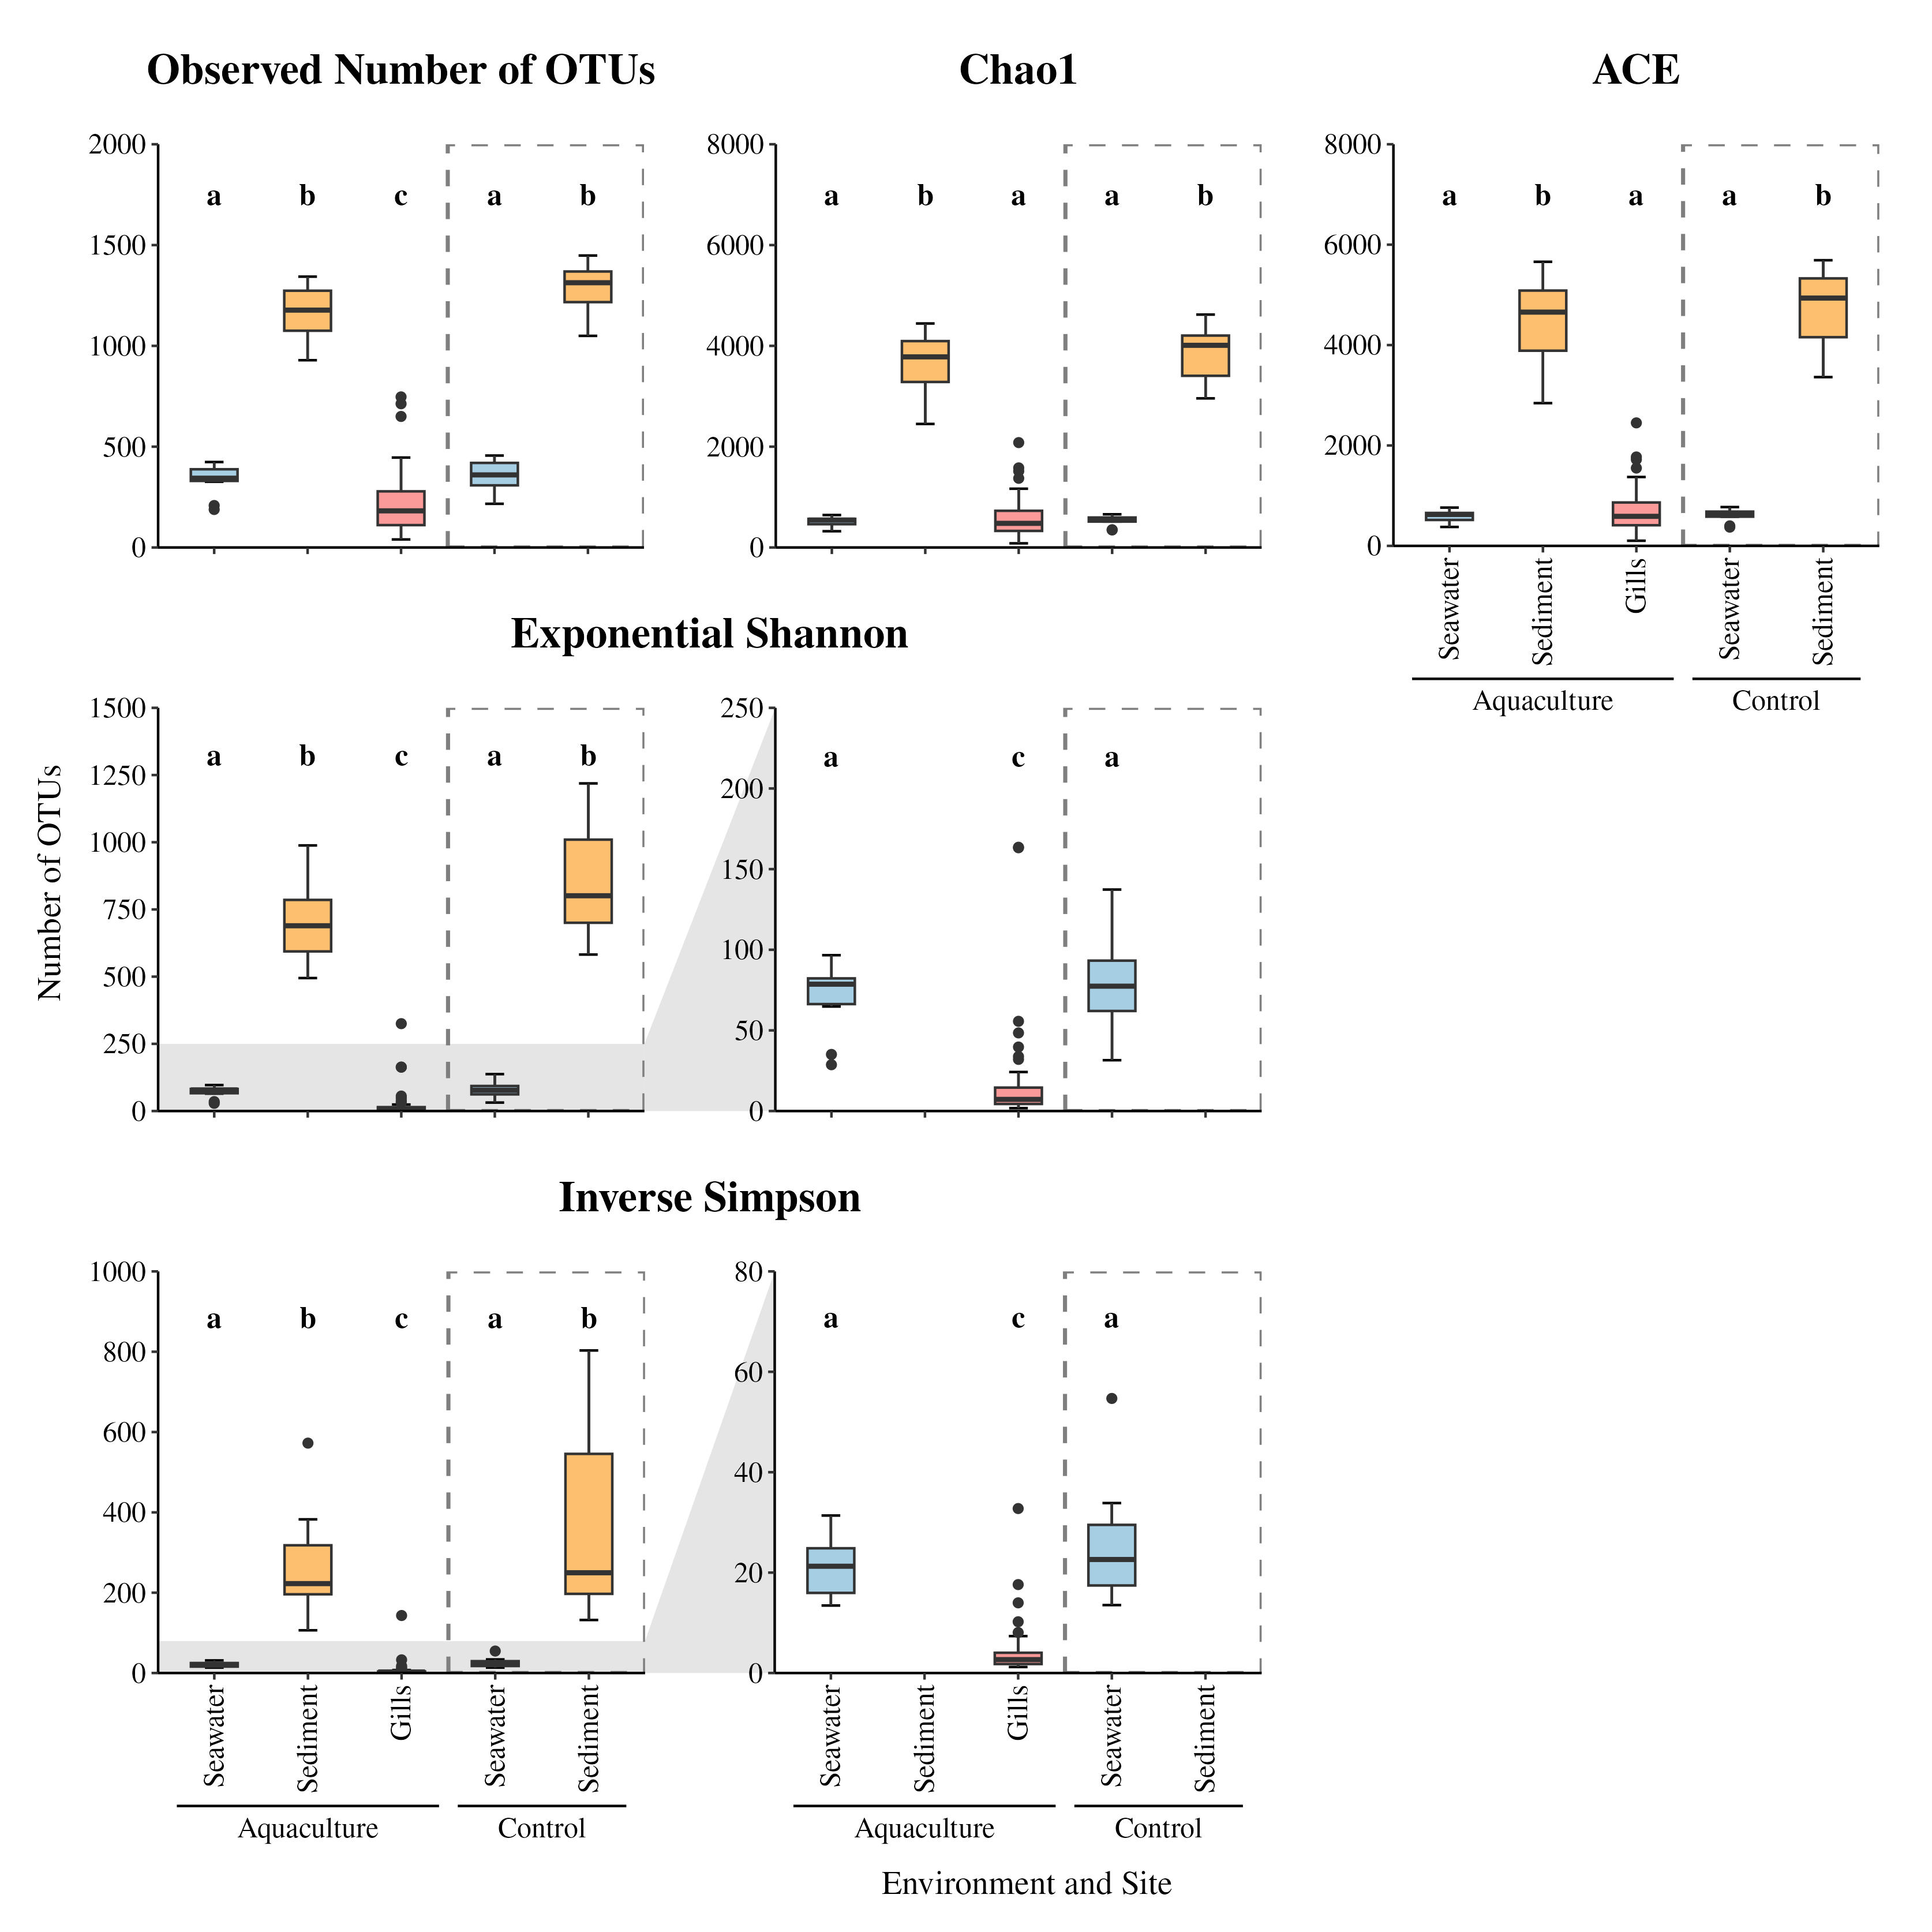
\includegraphics[width=0.9\linewidth]{../results/figures/alpha} 

}

\caption{The observed number of OTUs, Chao1, ACE, exponential of the Shannon diversity index, and Inverse Simpson diversity index of microbial communities from different environments and sites. Dashed boxes indicate groups of samples from the control site, while non-dashed areas represent groups of samples from the aquaculture site. Groups that do not share a letter are significantly different (\emph{p} \textless{} 0.05). Diagrams representing the exponential of the Shannon diversity index and the Inverse Simpson diversity index consist of a main panel showing the complete dataset and a magnified panel illustrating more clearly the differences between the microbial communities from seawater and from the gills of the mussel \emph{M. galloprovincialis} (gill microbiome)}\label{fig:alpha}
\end{figure}



\begin{figure}[t!]

{\centering 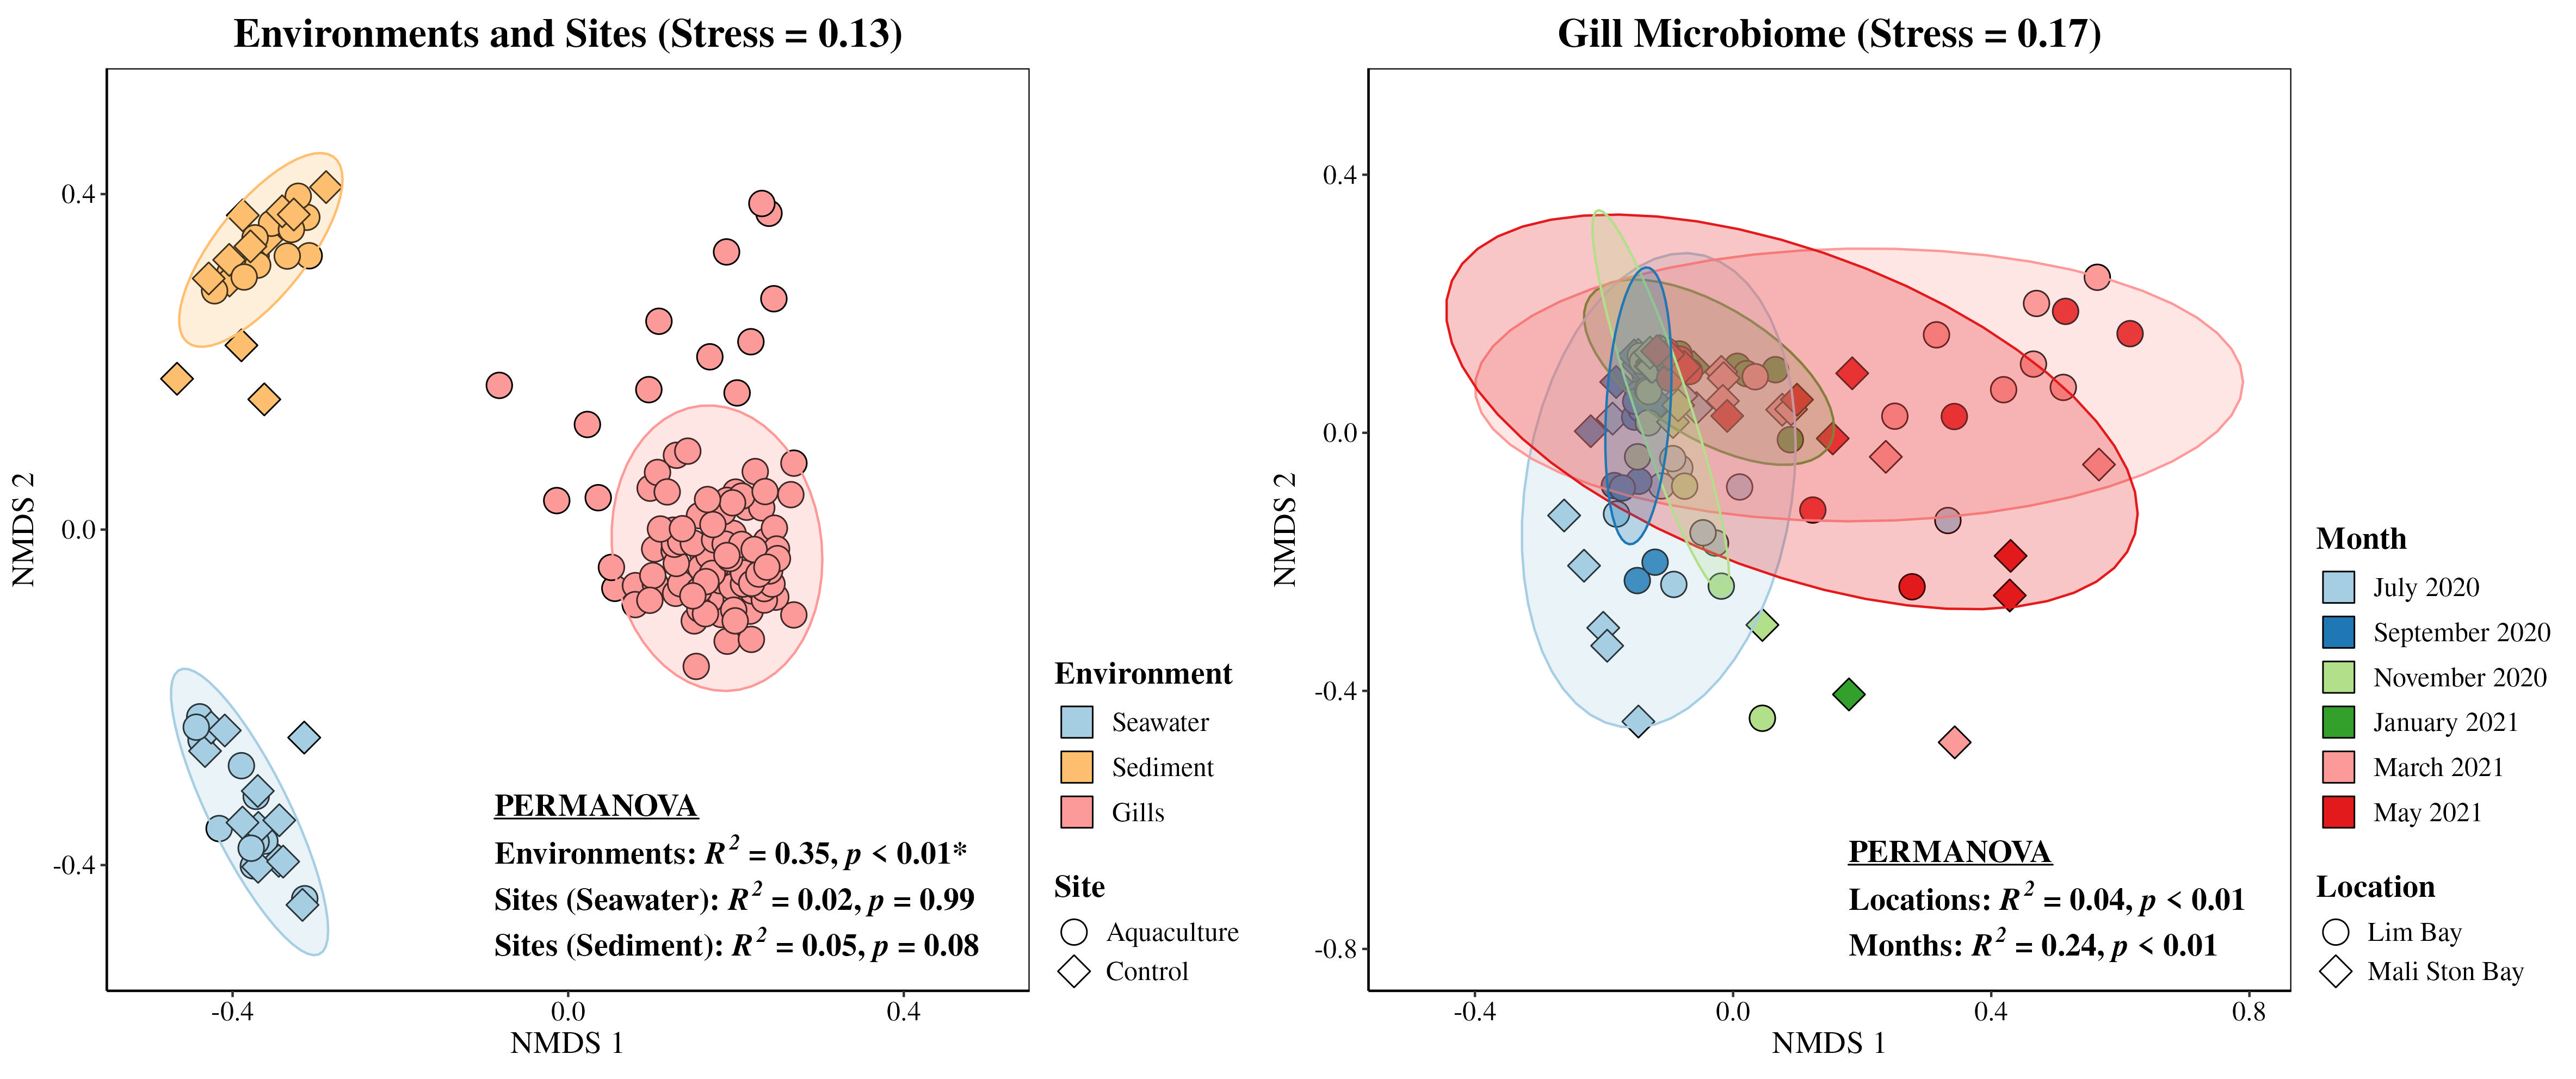
\includegraphics[width=1\linewidth]{../results/figures/nmds} 

}

\caption{NMDS of Bray--Curtis dissimilarities calculated from OTU abundances in microbial communities from different environments and sites, and in microbial communities from the gills of the mussel \emph{M. galloprovincialis} (gill microbiome) sampled in different months in both Lim Bay and Mali Ston Bay. The stress value for each NMDS is given in the corresponding plot title in parentheses. Ellipses represent 95\unit{\percent} confidence intervals for each environment and sampling month. PERMANOVA test results for differences between microbial communities from different environments, sites, sampling months, and locations are shown in the corresponding plots. *significant differences in the homogeneity of group dispersions (\emph{p} \textless{} 0.05) with unequal group sizes}\label{fig:nmds}
\end{figure}



To assess variation in the structure of microbial communities, Bray--Curtis dissimilarities based on OTU abundances were calculated and analysed using NMDS (Fig. \ref{fig:nmds}). When all samples were analysed together, a pronounced and statistically significant distinction between communities from different environments was observed (PERMANOVA, \emph{R\textsuperscript{2}} = 0.35, \emph{p} \textless{} 0.01, significant differences in the homogeneity of group dispersions {[}\emph{p} \textless{} 0.05{]} with unequal group sizes). Pairwise comparisons also showed significant differentiation among all environments (pairwise PERMANOVA, \emph{R\textsuperscript{2}} = 0.25--0.30, all \emph{p} \textless{} 0.01, Bonferroni-corrected). In contrast, there was no significant distinction in seawater (PERMANOVA, \emph{R\textsuperscript{2}} = 0.02, \emph{p} = 0.99) or sediment (PERMANOVA, \emph{R\textsuperscript{2}} = 0.05, \emph{p} = 0.08) communities between aquaculture and control sites (Fig. \ref{fig:nmds}). When the influence of sampling location, Lim Bay and Mali Ston Bay, was assessed, sediment microbial communities exhibited significant location-specific differentiation, with some community overlap (PERMANOVA, \emph{R\textsuperscript{2}} = 0.11, \emph{p} \textless{} 0.01). In contrast, seawater microbial communities did not show significant differentiation between locations (PERMANOVA, \emph{R\textsuperscript{2}} = 0.06, \emph{p} = 0.17), while location-specific differentiation of gill microbiomes was significant but almost negligible (PERMANOVA, \emph{R\textsuperscript{2}} = 0.04, \emph{p} \textless{} 0.01; Fig. \ref{fig:nmds}). When the influence of sampling month on the gill microbiome was assessed, significant temporal differentiation was observed (PERMANOVA, \emph{R\textsuperscript{2}} = 0.24, \emph{p} \textless{} 0.01, samples from January 2021 were excluded to avoid unequal group sizes; Fig. \ref{fig:nmds}). Pairwise comparisons showed significant differentiation among all months (pairwise PERMANOVA, \emph{R\textsuperscript{2}} = 0.12--0.29, all \emph{p} \textless{} 0.05, Bonferroni-corrected, samples from January 2021 were excluded to avoid unequal group sizes), except between September and November 2020 (pairwise PERMANOVA, \emph{R\textsuperscript{2}} = 0.05, \emph{p} = 0.61, Bonferroni-corrected) and between March and May 2021 (pairwise PERMANOVA, \emph{R\textsuperscript{2}} = 0.04, \emph{p} = 1.00, Bonferroni-corrected).

To compare the taxonomic composition of microbial communities between the sampled environments and sites, the average relative contribution of each taxon across samples from both locations and all sampling months was calculated (Fig. \ref{fig:taxonomy-environments-sites}). Differences in community structure between environments and similarities between sites identified by the NMDS were also evident in the taxonomic composition of the microbial communities. There were no notable differences between the aquaculture and control sites for the sediment and seawater communities. The seawater microbial community was mainly composed of the bacterial taxa \emph{Alphaproteobacteria} (aquaculture, 12.8--39.0\unit{\percent}; control, 11.1--42.1\unit{\percent}), \emph{Gammaproteobacteria} (aquaculture, 14.6--34.6\unit{\percent}; control, 13.4--32.7\unit{\percent}), \emph{Bacteroidota} (aquaculture, 7.5--19.3\unit{\percent}; control, 8.4--20.3\unit{\percent}), \emph{Cyanobacteriota} (aquaculture, 1.0--23.2\unit{\percent}; control, 1.2--21.6\unit{\percent}), \emph{Verrucomicrobiota} (aquaculture, 0.7--25.9\unit{\percent}; control, 0.8--24.5\unit{\percent}), and the archaeal phylum \emph{Thermoplasmatota} (aquaculture, 0.01--32.2\unit{\percent}; control, 0--32.5\unit{\percent}). The sediment microbial community differed from the seawater community and was mainly composed of the bacterial taxa \emph{Gammaproteobacteria} (aquaculture, 12.6--22.5\unit{\percent}; control, 11.1--24.7\unit{\percent}), \emph{Thermodesulfobacteriota} (aquaculture, 8.3--16.7\unit{\percent}; control, 2.0--16.6\unit{\percent}), \emph{Planctomycetota} (aquaculture, 9.8--15.3\unit{\percent}; control, 7.4--15.2\unit{\percent}), \emph{Bacteroidota} (aquaculture, 4.1--11.1\unit{\percent}; control, 2.9--15.8\unit{\percent}), \emph{Chloroflexota} (aquaculture, 3.3--7.2\unit{\percent}; control, 1.3--7.0\unit{\percent}), members without known relatives within \emph{Bacteria} (aquaculture, 2.5--13.1\unit{\percent}; control, 3.7--18.0\unit{\percent}), and the archaeal phylum \emph{Thermoproteota} (aquaculture, 1.6--13.1\unit{\percent}; control, 0.5--12.0\unit{\percent}; Fig. \ref{fig:taxonomy-environments-sites}). In contrast to the taxonomic composition of both the seawater and sediment microbial communities, the gill microbiome was largely composed of the bacterial class \emph{Gammaproteobacteria} (aquaculture, 27.0--98.8\unit{\percent}), while the proportions of other high-rank bacterial groups, such as \emph{Alphaproteobacteria} (aquaculture, 0.2--33.7\unit{\percent}), \emph{Bacteroidota} (aquaculture, 0.2--50.4\unit{\percent}), \emph{Planctomycetota} (aquaculture, 0.02--8.3\unit{\percent}), \emph{Bacillota} (aquaculture, 0.03--26.2\unit{\percent}) or members without known relatives within \emph{Bacteria} (aquaculture, 0.1--13.1\unit{\percent}), were substantially lower (Fig. \ref{fig:taxonomy-environments-sites}). The high proportion of \emph{Gammaproteobacteria} in the gill microbiome was observed in individuals at both locations and throughout the study period (Fig. \ref{fig:taxonomy-gills-phylum}), while \emph{Alphaproteobacteria}, \emph{Bacteroidota}, and \emph{Bacillota} comprised a notable proportion of the gill microbiome only in a few individuals (Supplementary Fig. \ref{supp-fig:taxonomy-gills-phylum-without-gammaproteobacteria}).

\begin{figure}[t!]

{\centering 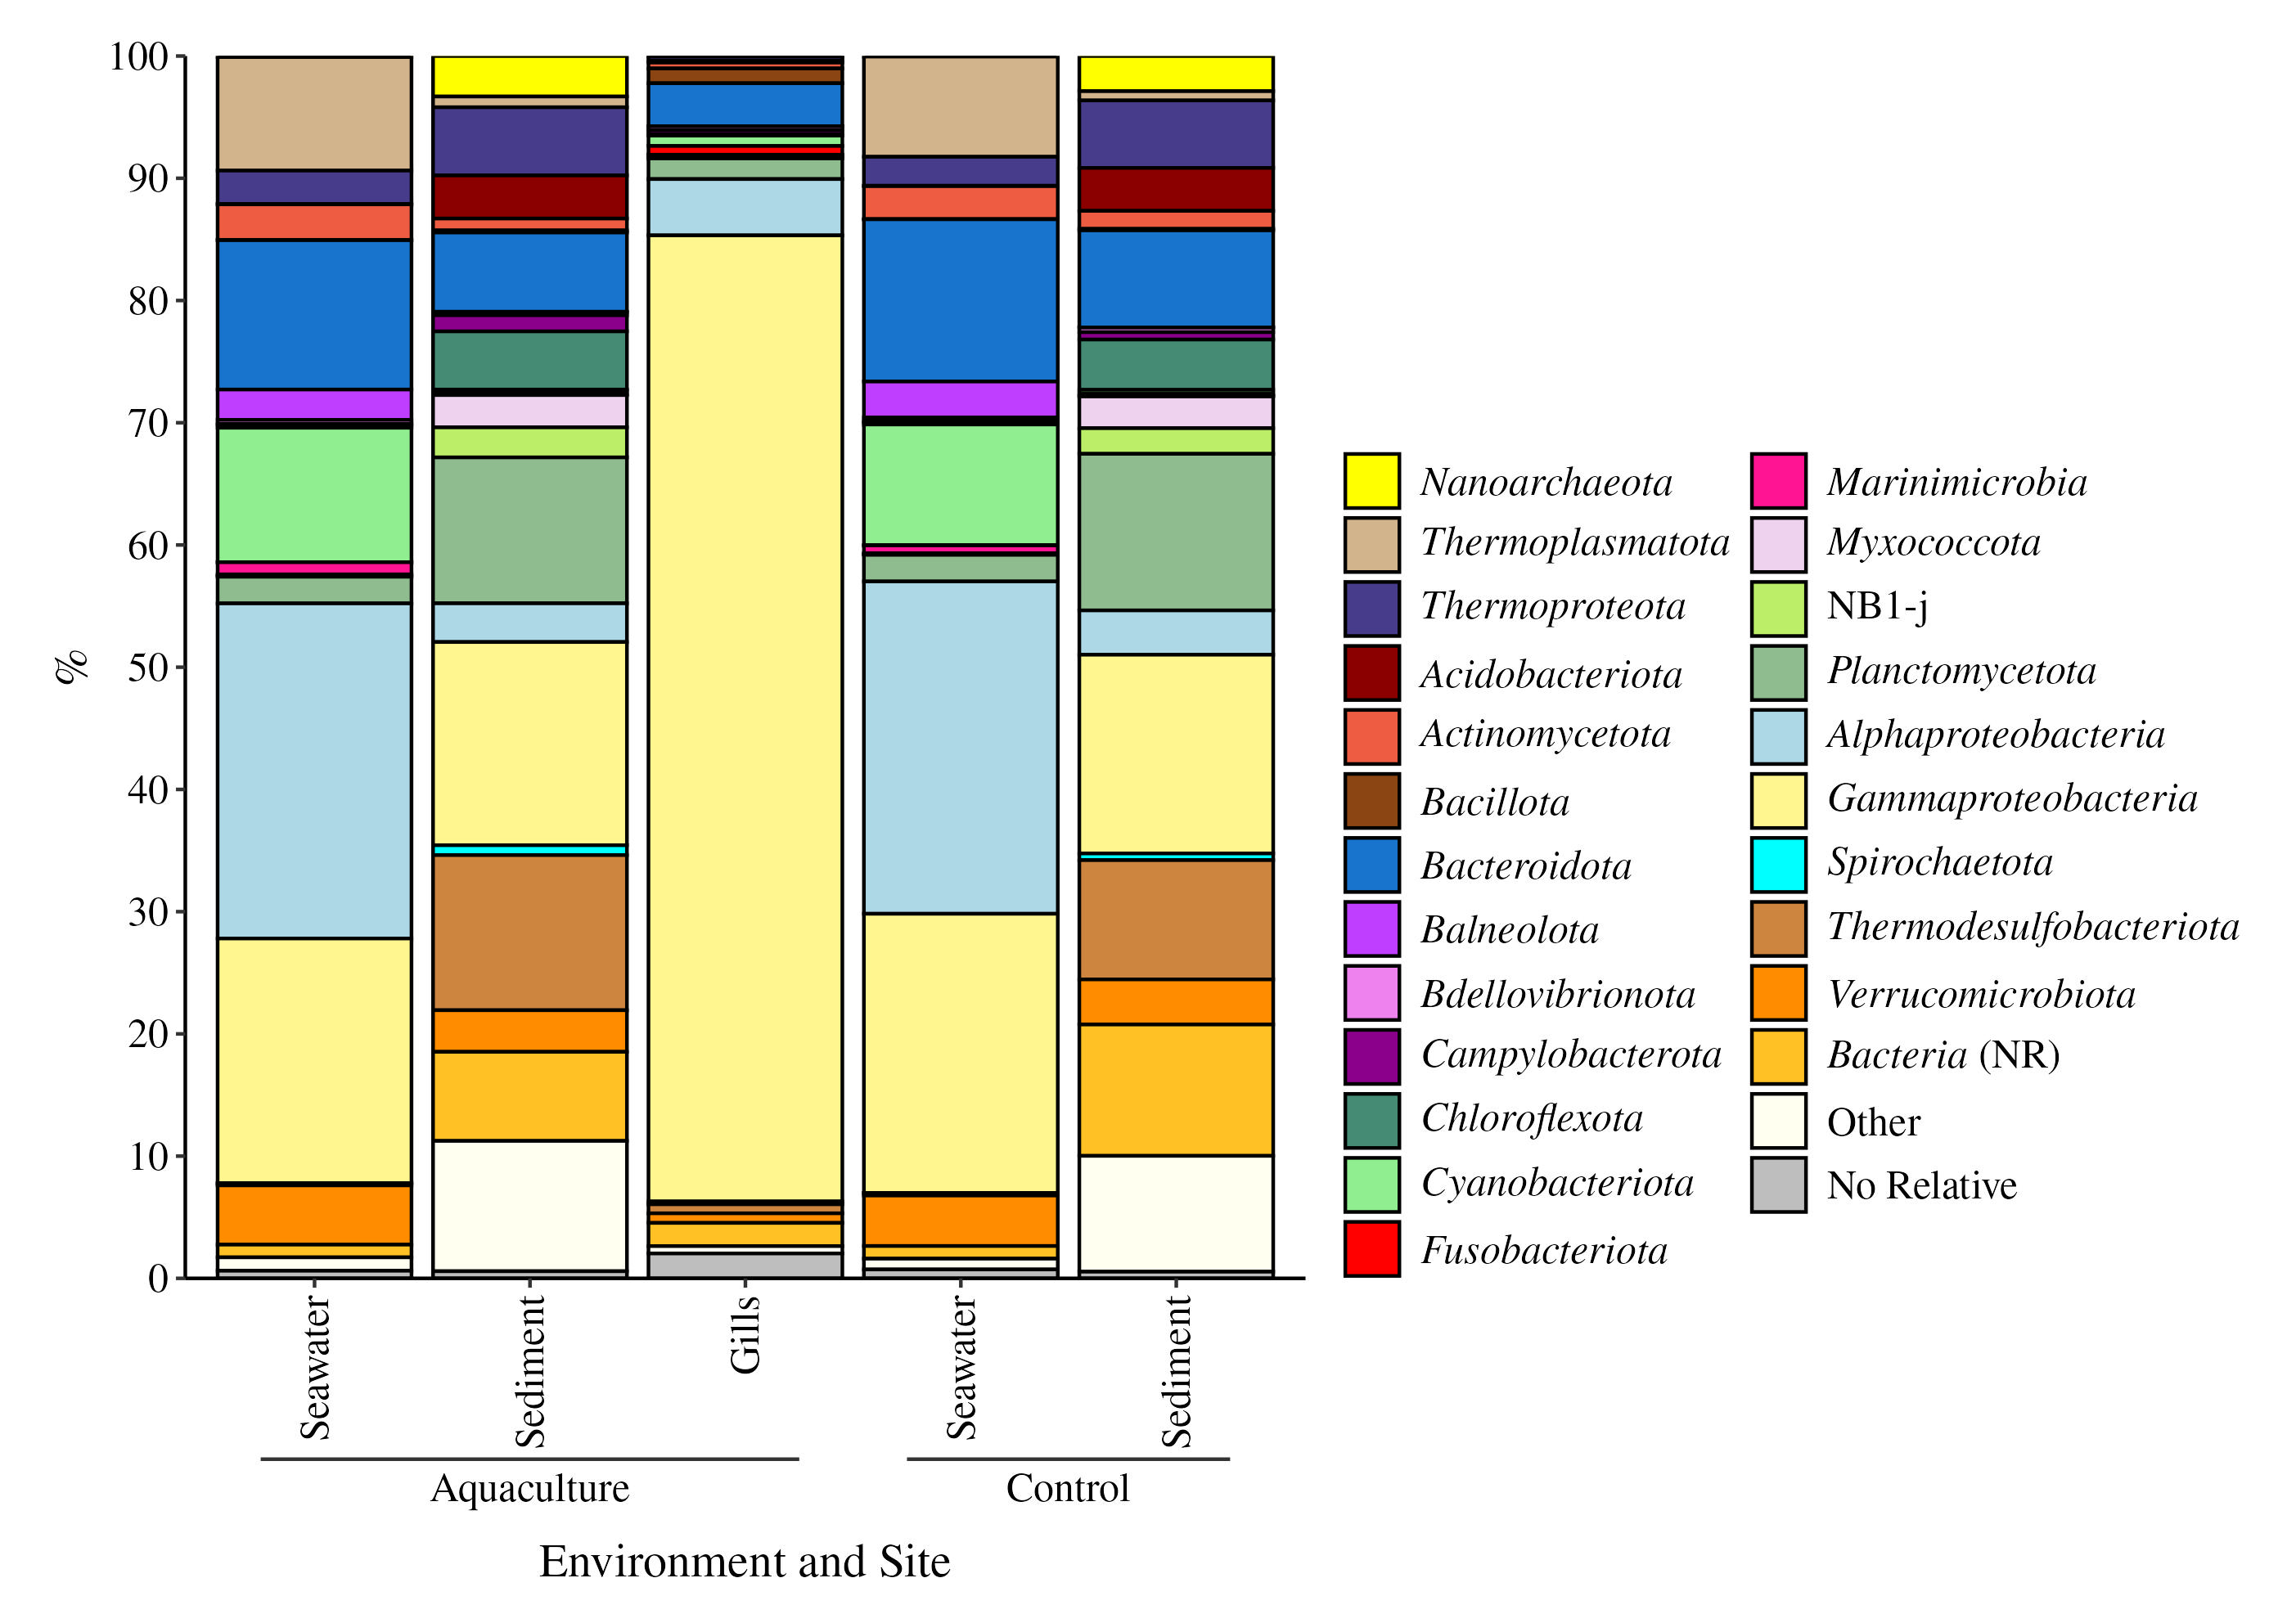
\includegraphics[width=1\linewidth]{../results/figures/taxonomy_environments_sites} 

}

\caption{Taxonomic classification and average relative contribution of the most abundant (\qty{>=3}{\percent}) bacterial and archaeal sequences in different sampled environments and at each site. The average relative contribution of each taxon across samples from both Lim Bay and Mali Ston Bay, and across all sampling months, was calculated. ``No Relative'' indicates sequences that could not be classified into any taxon, while ``NR'' (No Relative) next to the name of a taxonomic group refers to sequences that could not be assigned to any known taxon within that group}\label{fig:taxonomy-environments-sites}
\end{figure}



\begin{figure}[t!]

{\centering 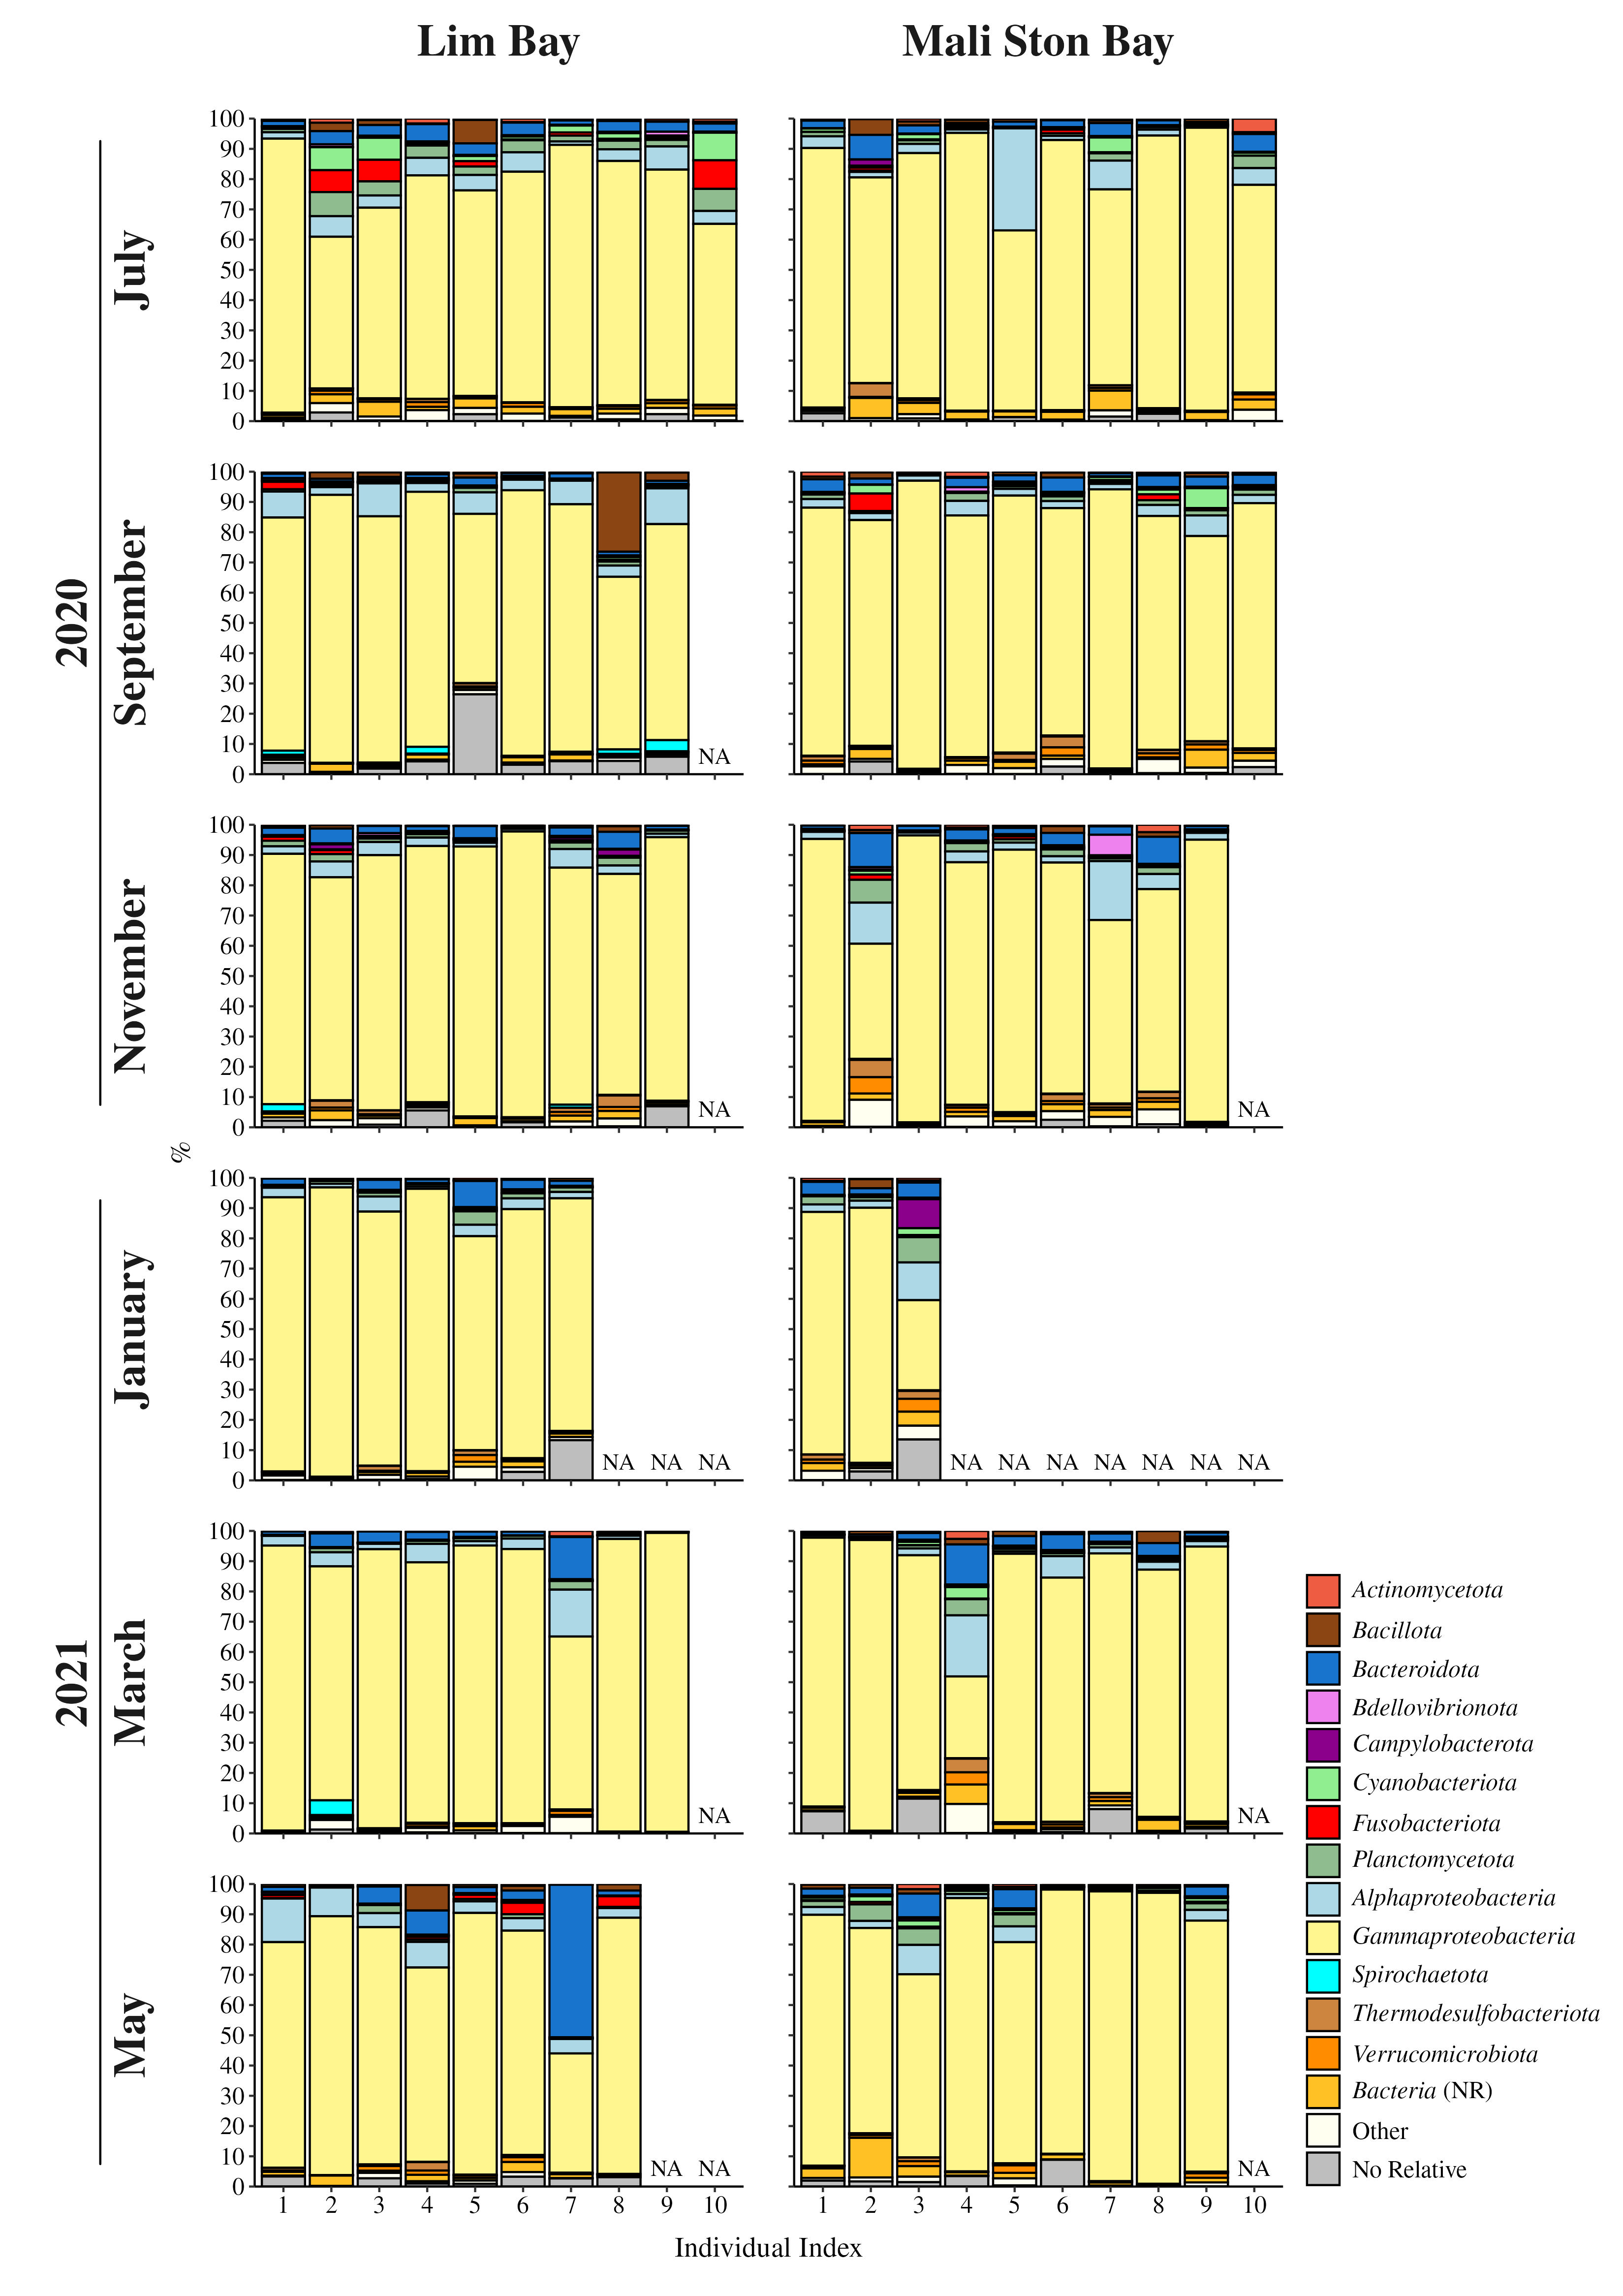
\includegraphics[width=0.7\linewidth]{../results/figures/taxonomy_gills_phylum} 

}

\caption{Taxonomic classification and relative contribution of the most abundant (\qty{>=3}{\percent}) bacterial and archaeal sequences from the gills of the mussel \emph{M. galloprovincialis} (gill microbiome). From July 2020 to May 2021, 10 mussels were collected per sampling month in Lim Bay and Mali Ston Bay. Each bar (individual index) represents an individual mussel (see Supplementary Table \ref{supp-tab:nseq-notus-gills}). ``No Relative'' indicates sequences that could not be classified into any taxon, while ``NR'' (No Relative) next to the name of a taxonomic group refers to sequences that could not be assigned to any known taxon within that group. ``NA'' (Not Available) indicates samples that were not successfully analysed}\label{fig:taxonomy-gills-phylum}
\end{figure}



A more detailed analysis of the taxonomic composition of the seawater microbial community revealed temporal patterns for some taxa (Supplementary Fig. \ref{supp-fig:taxonomy-seawater-sediment-phylum}). For example, the archaeal phylum \emph{Thermoplasmatota} showed a similar pattern at both locations and sites, comprising a higher proportion of the community from November 2020 to January 2021 (10.9--32.5\unit{\percent}) than in other months (0--4.6\unit{\percent}). Notably, during the months when the proportion of this archaeal phylum was high, almost the entire \emph{Thermoplasmatota} community consisted of Marine Group II (95.2--100\unit{\percent}). Marked differences between locations were observed in May 2021, when in Lim Bay at both sites, more than half of the microbial community was composed of \emph{Gammaproteobacteria} (31.5--34.6\unit{\percent}) and \emph{Verrucomicrobiota} (24.5--25.9\unit{\percent}), which was higher than in Mali Ston Bay at the same time (\emph{Gammaproteobacteria}, 20.2--23.6\unit{\percent}; \emph{Verrucomicrobiota}, 3.9--3.9\unit{\percent}) or in other months (\emph{Gammaproteobacteria}, 13.4--32.7\unit{\percent}; \emph{Verrucomicrobiota}, 0.7--4.7\unit{\percent}). In contrast, \emph{Alphaproteobacteria} constituted a lower proportion of the microbial community in Lim Bay in May 2021 (11.1--12.8\unit{\percent}) than in Mali Ston Bay at the same time (31.0--39.0\unit{\percent}) or in other months (19.6--42.1\unit{\percent}). For the sediment microbial community, a fairly similar taxonomic composition between locations and sites, as well as across sampling months, was observed (Supplementary Fig. \ref{supp-fig:taxonomy-seawater-sediment-phylum}). The only notable exception was the sediment community in Mali Ston Bay at the control site, where, for example, \emph{Thermodesulfobacteriota} comprised a lower proportion of the community from July to November 2020 (2.0--5.1\unit{\percent}) than from January to May 2021 (10.8--16.6\unit{\percent}). This low proportion of \emph{Thermodesulfobacteriota} was also lower than that observed at the aquaculture site in Mali Ston Bay (9.9--16.7\unit{\percent}) and at both sites in Lim Bay (8.3--15.2\unit{\percent}).

\begin{figure}[t!]

{\centering 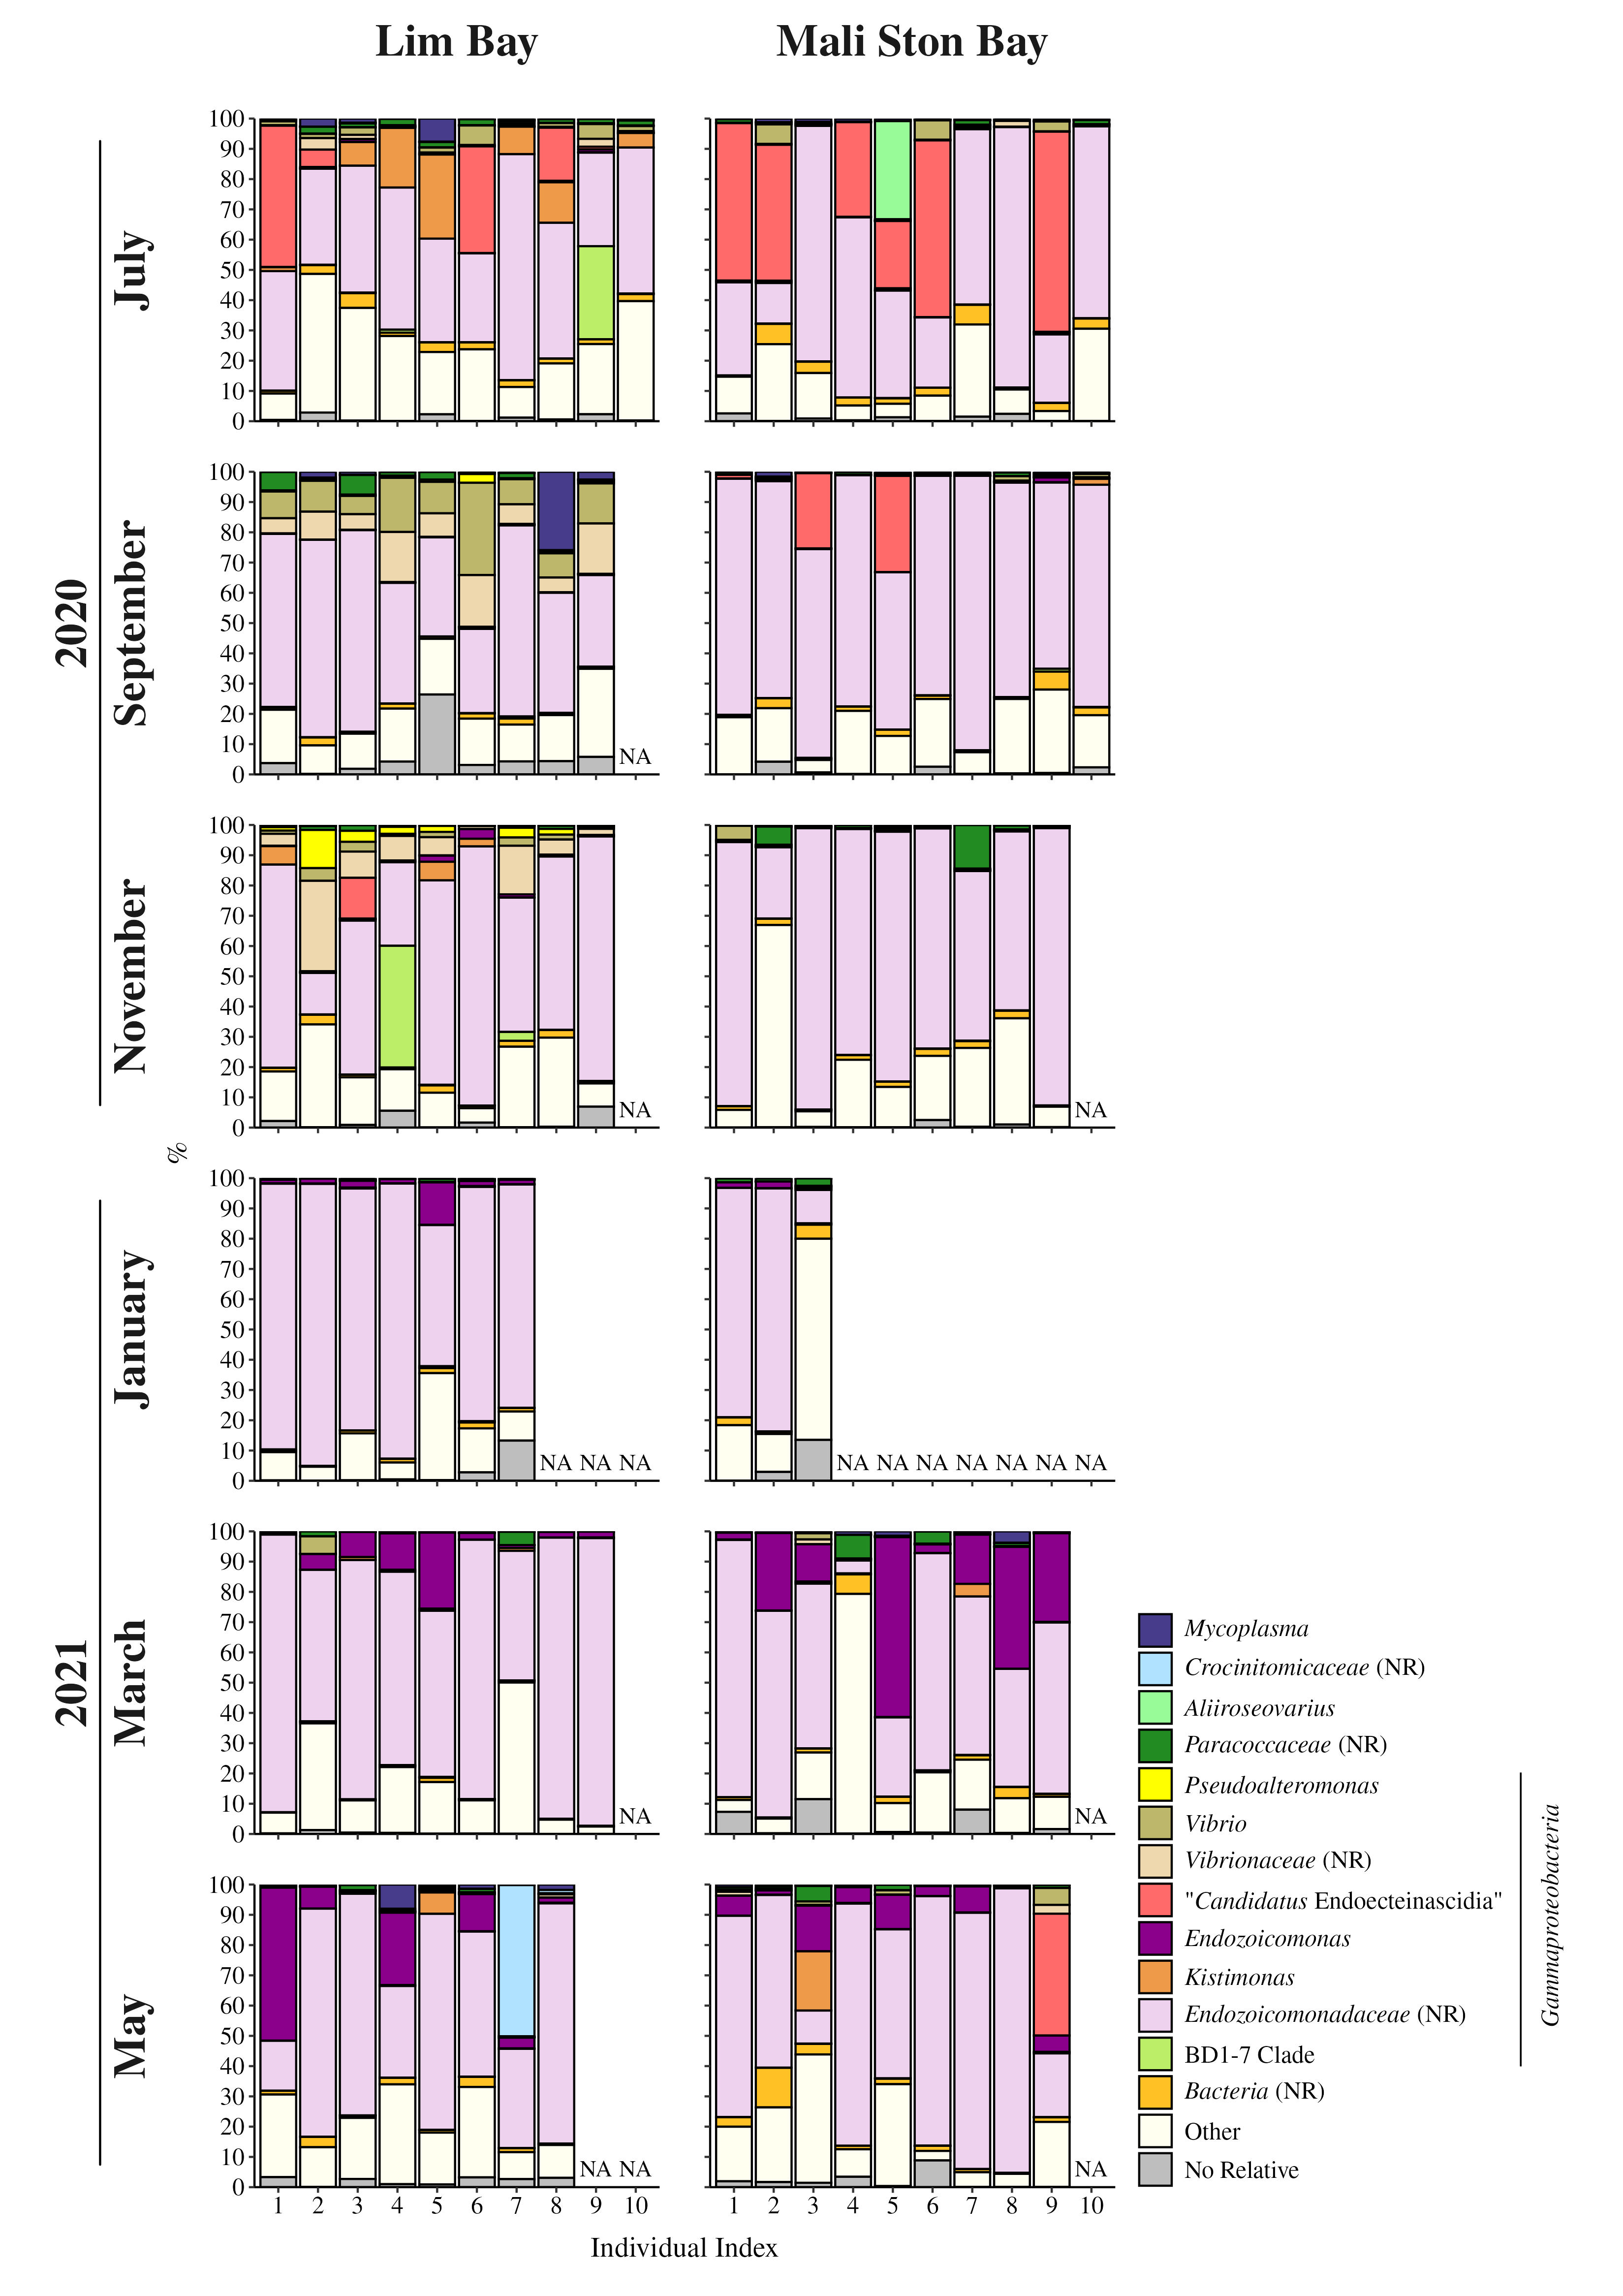
\includegraphics[width=0.7\linewidth]{../results/figures/taxonomy_gills_genus} 

}

\caption{Relative contribution of the most abundant (\qty{>=10}{\percent}) bacterial and archaeal sequences from the gills of the mussel \emph{M. galloprovincialis} (gill microbiome) classified at the genus taxonomic rank. From July 2020 to May 2021, 10 mussels were collected per sampling month in Lim Bay and Mali Ston Bay. Each bar (individual index) represents an individual mussel (see Supplementary Table \ref{supp-tab:nseq-notus-gills}). ``No Relative'' indicates sequences that could not be classified into any taxon, while ``NR'' (No Relative) next to the name of a taxonomic group refers to sequences that could not be assigned to any known taxon within that group. ``NA'' (Not Available) indicates samples that were not successfully analysed}\label{fig:taxonomy-gills-genus}
\end{figure}



Because, as previously mentioned, the gill microbiome of most \emph{M. galloprovincialis} mussels, except for a few individuals, was largely composed of \emph{Gammaproteobacteria}, no differences in community composition between locations or sampling months were identified (Fig. \ref{fig:taxonomy-gills-phylum}). However, when the taxonomic composition was analysed at lower taxonomic ranks, such as family and genus, differences between locations and sampling months were observed (Fig. \ref{fig:taxonomy-gills-genus}). Although high variability in the taxonomic composition of each individual's gill microbiome was noted, low-rank gammaproteobacterial groups present at both locations and throughout the study period, as well as groups specific to certain locations or months, were identified. In addition to these patterns, samples that did not yield sufficient sequences for further analysis were also specific to a particular month, January 2021, when 10 samples did not yield sufficient sequences, whereas in all other months only eight samples lacked enough sequences for further analysis (Figs. \ref{fig:taxonomy-gills-phylum} and \ref{fig:taxonomy-gills-genus}). Members without known relatives within \emph{Endozoicomonadaceae} were present in mussel gills at both locations and throughout the study period, showing a high degree of variability between individuals (4.3--95.1\unit{\percent}; Fig. \ref{fig:taxonomy-gills-genus}). When differences in the proportion of this group between individuals from different locations were tested, the only significant difference was its higher proportion in the gill microbiome of individuals from Mali Ston Bay (52.0--90.7\unit{\percent}) compared to those from Lim Bay (27.9--66.6\unit{\percent}) in September 2020 (Mann--Whitney \emph{U} test, \emph{p} \textless{} 0.001, testing for January 2021 was omitted because of the limited number of samples). In addition, significant differences between months were observed only in Lim Bay (Kruskal--Wallis \emph{H} test, \emph{p} \textless{} 0.01, samples from Mali Ston Bay from January 2021 were excluded due to the limited number of samples), specifically between July 2020 (29.4--74.7\unit{\percent}) and January 2021 (46.7--93.2\unit{\percent}), July 2020 and March 2021 (42.9--95.1\unit{\percent}), and between September 2020 (27.9--66.6\unit{\percent}) and January 2021 (pairwise Mann--Whitney \emph{U} test, all stated comparisons \emph{p} \textless{} 0.05, Bonferroni-corrected). Interestingly, \emph{Endozoicomonas}, a member of the family \emph{Endozoicomonadaceae}, was almost absent in the gill microbiome at both locations from July to November 2020 (0--3.2\unit{\percent}), but from January to May 2021 it comprised a substantial proportion of the microbiome in many individuals from both locations (0.5--59.5\unit{\percent}; Mann--Whitney \emph{U} test, \emph{p} \textless{} 0.0001; Fig. \ref{fig:taxonomy-gills-genus}). Another taxonomic group showing specificity to a certain period was ``\emph{Candidatus} Endoecteinascidia'', which comprised a substantial proportion of the gill microbiome in many individuals in July 2020 (0--66.1\unit{\percent}), while in other months the microbiomes of only a few individuals contained a higher proportion of this group (0--40.3\unit{\percent}; Fig. \ref{fig:taxonomy-gills-genus}). These differences in proportions of ``\emph{Candidatus} Endoecteinascidia'' between July 2020 and all other months were supported by the Mann--Whitney \emph{U} test (all \emph{p} \textless{} 0.01, Bonferroni-corrected). \emph{Vibrio} showed differences in the proportion of the gill microbiome between locations and sampling months (Fig. \ref{fig:taxonomy-gills-genus}). In September 2020, higher proportions of this group were observed in gill microbiomes from Lim Bay (6.0--30.5\unit{\percent}) than from Mali Ston Bay (0.1--1.5\unit{\percent}). In addition, these proportions in September 2020 were also higher than those observed in all other months at either location (0--6.5\unit{\percent}). These differences in the proportion of the gill microbiome between individuals from Lim Bay in September 2020 and individuals from all other months at either location were supported by the Mann--Whitney \emph{U} test (all \emph{p} \textless{} 0.01, Bonferroni-corrected, samples from Mali Ston Bay from January 2021 were excluded due to the limited number of samples). Furthermore,
members without known relatives within \emph{Vibrionaceae} also showed differences in the proportion of the gill microbiome between locations and sampling months (Fig. \ref{fig:taxonomy-gills-genus}). Higher proportions of this group were observed in individuals from Lim Bay in September (4.9--17.1\unit{\percent}) and November (1.0--29.9\unit{\percent}) 2020 than in individuals from Mali Ston Bay in the same months (September 2020, 0.008--0.3\unit{\percent}; November 2020, 0.06--0.5\unit{\percent}). In addition, these proportions in individuals from Lim Bay from September to November 2020 were also higher than those observed in individuals from all other months at either location (0--3.8\unit{\percent}). The similarities in proportions of this group in individuals from Lim Bay in September and November 2020 and the differences from individuals from all other months at either location were supported by the Mann--Whitney \emph{U} test (all \emph{p} \textless{} 0.01, Bonferroni-corrected, samples from Mali Ston Bay from January 2021 were excluded due to the limited number of samples). Additionally, the relationship between members without known relatives within \emph{Vibrionaceae} and \emph{Vibrio} was assessed in individuals from Lim Bay in September 2020, when both groups showed higher proportions (Fig. \ref{fig:taxonomy-gills-genus}). This assessment indicated that members without known relatives within \emph{Vibrionaceae} accounted for 36.0--55.7\unit{\percent} of their combined contribution.

The presence of taxa abundant in the gill microbiome (members without known relatives within \emph{Endozoicomonadaceae}, \emph{Endozoicomonas}, ``\emph{Candidatus} Endoecteinascidia'', \emph{Vibrio}, and members without known relatives within \emph{Vibrionaceae}) was also assessed in seawater (23 samples in total) and sediment (24 samples in total) microbial communities to evaluate the influence of microbes from these surrounding environments on the gill microbiome. Members without known relatives within \emph{Endozoicomonadaceae} were detected in only three seawater and four sediment samples, and at very low proportions (seawater, 0.02--0.03\unit{\percent}; sediment, 0.007--0.06\unit{\percent}). \emph{Endozoicomonas} was detected in nine sediment samples, again at very low proportions (0.005--0.1\unit{\percent}), whereas ``\emph{Candidatus} Endoecteinascidia'' was observed only in five seawater samples, also at very low proportions (0.03--0.2\unit{\percent}). \emph{Vibrio} and members without known relatives within \emph{Vibrionaceae} were detected in more seawater and sediment samples. \emph{Vibrio} was present in 10 seawater and 14 sediment samples, at proportions of 0.03--0.7\unit{\percent} in the seawater community and 0.005--1.3\unit{\percent} in the sediment community. Similarly, members without known relatives within \emph{Vibrionaceae} occurred in 13 seawater and eight sediment samples, with proportions of 0.03--2.0\unit{\percent} in the seawater community and 0.008--0.2\unit{\percent} in the sediment community. The presence or absence of these taxa in seawater and sediment samples from specific locations or sampling months could not be associated with their high proportions in the gill microbiome at the same locations and months.
\newpage

\section{Discussion}\label{discussion}

The mussel \emph{M. galloprovincialis} is a filter-feeding animal, meaning that, as in most bivalve species, its gills are used for both gas exchange and feeding {[}\citeproc{ref-Gosling2003a}{37}{]}. More specifically, it is a suspension-feeding bivalve that relies on the selective uptake of seston, comprising living and non-living material across a wide size range, to acquire suspended particles used as a food source, such as phytoplankton, microzooplankton, microbes, and detritus {[}\citeproc{ref-Rosa2018}{38}, \citeproc{ref-Ward2004}{39}, \citeproc{ref-Gosling2003c}{96}{]}. The flow of seawater required for feeding is generated by lateral cilia on the gills. Seawater flows through the inhalant aperture, passes through the interfilamentary spaces of the gills into the suprabranchial cavity, and exits through the exhalant aperture {[}\citeproc{ref-Rosa2018}{38}, \citeproc{ref-Ward2004}{39}{]}. Food particles are retained by the gills whose capture efficiency depends on particle size, with smaller particles, such as free-living microbes, being less likely to be retained than larger ones, including particle-attached microbes. Captured particles are then selectively processed by mucociliary mechanisms and are either ingested or rejected as pseudofaeces {[}\citeproc{ref-Rosa2018}{38}, \citeproc{ref-Ward2004}{39}, \citeproc{ref-Ward1996}{97}, \citeproc{ref-Ward1998}{98}{]}. As the gills, which are essential for this suspension-feeding mechanism, must be in relatively constant contact with seawater and may also be influenced by material resuspended from the seafloor {[}\citeproc{ref-Rosa2018}{38}, \citeproc{ref-Ward2004}{39}, \citeproc{ref-Asmus2011}{47}, \citeproc{ref-Velasco2005}{48}{]}, it is therefore appropriate to compare the gill microbiome with the microbial communities in the surrounding seawater and sediment.

In this study, the observed number of OTUs, as well as the exponential of the Shannon diversity index and the Inverse Simpson diversity index, were significantly lower for the gill microbiome than for the seawater and sediment microbial communities. However, when the total number of OTUs is considered using calculated richness estimators, the difference in the number of OTUs between the gill microbiome and the seawater microbial community is no longer evident. This lower observed number of OTUs in the gill microbiome compared with the seawater microbial community, together with the absence of differences in the predicted number of OTUs based on richness estimators, is likely due to the mussel selectively excluding many rare seawater OTUs from its gill microbiome. A study on the gill microbiome of the same species reported differences in alpha diversity between the gill microbiome and the microbial community in the surrounding seawater {[}\citeproc{ref-Zardinoni2024}{31}{]}, while another study found no differences between the microbial community in the surrounding seawater and the microbiome of various body parts of this species, including the gills {[}\citeproc{ref-Musella2020}{14}{]}. In any case, the alpha diversity of the gill microbiome and seawater microbial community was substantially lower than that of the sediment community. Similarly, comparisons of the gut and shell microbiome of the eastern oyster, \emph{Crassostrea virginica}, with the sediment microbial community also found lower alpha diversity in the oyster's gut and shell microbiome than in the sediment community {[}\citeproc{ref-Arfken2017}{12}{]}. The alpha diversity of the gill microbiome did not differ between the two locations, Lim Bay and Mali Ston Bay, consistent with a study comparing the gill microbiome of \emph{M. galloprovincialis} between nearby locations {[}\citeproc{ref-Zardinoni2024}{31}{]}, as well as another study comparing its whole microbiome between more distant geographic locations {[}\citeproc{ref-Peruzzo2026}{23}{]}. Richness estimators were also the only alpha diversity parameters showing significant overall differences in the gill microbiome between sampling months, although pairwise comparisons did not show any significant differences between individual months. Overall, it appears that the mussel \emph{M. galloprovincialis} has a gill microbiome with lower alpha diversity than the surrounding sediment microbial community, a lower observed number of OTUs and lower diversity indices than the community in the surrounding seawater, and no differences in predicted richness compared with the surrounding seawater community. In addition, its gill microbiome appears to be stable in terms of alpha diversity, showing minimal variation between different sampling locations and months.

Although richness estimators did not indicate differences between the gill microbiome of \emph{M. galloprovincialis} and the microbial community in the surrounding seawater, NMDS performed on Bray--Curtis dissimilarity calculated from OTU abundances revealed a clear separation between the gill microbiome and the communities in both the surrounding seawater and sediment. This finding is consistent with studies reporting differences between the microbiome of this species' various body parts, such as the gut, gills, and haemolymph, and the community in the surrounding seawater {[}\citeproc{ref-Akter2023}{11}, \citeproc{ref-Musella2020}{14}, \citeproc{ref-Vezzulli2018}{16}, \citeproc{ref-Palladino2023}{28}, \citeproc{ref-Zardinoni2024}{31}{]}, as well as with the distinct community structures observed between the gut and shell microbiomes of the eastern oyster and the microbial community in the surrounding sediment {[}\citeproc{ref-Arfken2017}{12}{]}. In addition, the high similarity of sediment microbial communities between the aquaculture and control sites suggests low spatial heterogeneity in sediment properties over short physical distances from mussel-growing structures. However, while local impacts were not detected at the small scale studied, a larger-scale study across a wider area may be needed to fully evaluate potential interactions between farmed bivalves with the benthic environment {[}\citeproc{ref-Tong2025}{99}{]}. Comparison of the overall structure of the \emph{M. galloprovincialis} gill microbiome at the OTU level in this study did not reveal significant differentiation between the two locations, Lim Bay and Mali Ston Bay, despite their considerable geographic distance. This agrees with a study of the gill microbiome of the same species that also did not show variation between locations {[}\citeproc{ref-Zardinoni2024}{31}{]}. In contrast, the structure of the gut microbiome of the same species varied with geographic location {[}\citeproc{ref-delRio-Lavin2023}{21}, \citeproc{ref-Palladino2023}{28}{]}, indicating a greater influence of local conditions on the gut than on the gill microbiome, possibly due to variation in the origin of food, which also includes microbes, with geographic location and the potential involvement of the gut microbiota in food digestion {[}\citeproc{ref-Pierce2018}{7}, \citeproc{ref-Gosling2003c}{96}{]}. Interestingly, the structure of the overall microbiome of the mussel \emph{M. galloprovincialis} transported from one geographic location to another is initially different and converges towards that of native mussels, highlighting the influence of local conditions, the possible high contribution of the gut microbiota to the overall microbiome, and the importance of assessing tissue-specific microbiomes {[}\citeproc{ref-Peruzzo2026}{23}{]}. Furthermore, in this study, the structure of the gill microbiome at the OTU level showed a separation of microbiomes from different sampling months, except between September and November 2020 and between March and May 2021, indicating the presence of microbiome taxa with temporal changes. Similarly, studies on the overall microbiome of the mussel \emph{M. galloprovincialis} {[}\citeproc{ref-Peruzzo2026}{23}{]}, as well as on the gut microbiome {[}\citeproc{ref-Akter2023}{11}, \citeproc{ref-Palladino2023}{28}, \citeproc{ref-Wathsala2021}{30}{]}, also indicated temporal microbiome changes. In contrast, a study of the gill microbiome of the same species did not reveal any temporal changes, possibly due to the fewer sampling months included in that study {[}\citeproc{ref-Zardinoni2024}{31}{]}.

Consistent with the NMDS analysis based on OTU abundances, the taxonomic analysis also revealed a clear distinction between the gill microbiome of the mussel \emph{M. galloprovincialis} and the communities in the surrounding seawater and sediment. The high-rank microbial taxa detected in the surrounding seawater, as well as the higher proportion of \emph{Thermoplasmatota} Marine Group II during the colder period of the year, are typical of seawater microbial communities in the Adriatic Sea {[}\citeproc{ref-Korlevic2015}{100}, \citeproc{ref-Korlevic2022}{101}{]}. Similarly, the high-rank microbial taxa detected in the surrounding sediment have previously been found in surface sediments of the Adriatic Sea {[}\citeproc{ref-Markovski2022}{50}, \citeproc{ref-Ramljak2024}{102}{]}. At higher taxonomic ranks, the distinction between the gill microbiome and the microbial communities in the surrounding seawater and sediment was mainly due to the high proportion of \emph{Gammaproteobacteria} in the gill microbiome. The high proportion of taxa belonging to this class in the gill microbiome has also been observed in other studies focusing on the gills of the mussel \emph{M. galloprovincialis} {[}\citeproc{ref-Musella2020}{14}, \citeproc{ref-Zardinoni2024}{31}{]}. Because of the high proportion of \emph{Gammaproteobacteria} in the gill microbiome, no differences between the two locations, Lim Bay and Mali Ston Bay, or between sampling months were observed. However, when the analysis was performed at lower taxonomic ranks, such as family and genus, taxa were identified that were either resident, based on their consistent presence at both locations and throughout the study period, or specific to certain locations or months, likely exhibiting transient associations with the mussel host. In addition, samples that did not yield sufficient sequences for further analysis were also specific to a particular month, namely January 2021. This peculiarity may be attributed to lower microbial counts in the gills in winter, as many microbes exhibit reduced growth at lower water temperatures, regardless of the bivalve host species or tissue {[}\citeproc{ref-Pierce2018}{7}, \citeproc{ref-Cavallo2009}{103}--\citeproc{ref-Sheikh2022}{105}{]}.

Although members without known relatives within \emph{Endozoicomonadaceae} showed high variability in their proportion within the gill microbiome of \emph{M. galloprovincialis} between individuals, they were detected in all analysed mussels, showed minimal differences in proportion between mussels from different locations or months, and were only sporadically detected at very low proportions in seawater. This suggests that this group may be regarded as putatively resident in the gills of \emph{M. galloprovincialis}. It is important to note that, although consistent detection of members of this group across a wider geographic area suggests a strong association with this host {[}\citeproc{ref-Unzueta-Martinez2022a}{8}{]}, applying methodologies to multiple bivalve host species that allow strain tracking, as well as approaches enabling the localisation of microbial cells in tissues, such as fluorescence in situ hybridisation (FISH), is crucial for verifying their residency {[}\citeproc{ref-daSilva2025}{106}--\citeproc{ref-Neave2016}{108}{]}. The family \emph{Endozoicomonadaceae} is known to form associations with many marine benthic invertebrates, including sponges and bivalves, as well as with some fishes {[}\citeproc{ref-Munoz-Martinez2026}{6}, \citeproc{ref-daSilva2025}{106}, \citeproc{ref-Hoy2026}{109}, \citeproc{ref-Schill2017}{110}{]}. Furthermore, members of this family have previously been detected in the gills of \emph{M. galloprovincialis} {[}\citeproc{ref-Cano2020}{111}{]}, as well as in the gills of \emph{Mytilus edulis} {[}\citeproc{ref-Schill2017}{110}{]} and \emph{Mytilus californianus} {[}\citeproc{ref-Neu2021}{112}{]}, two bivalve species related to \emph{M. galloprovincialis}. Genomic analyses suggest that members of this family can rapidly adapt and transition between free-living and host-associated lifestyles, resulting in host--microbe relationships that can range from mutualistic to parasitic depending on the host species and ecological context {[}\citeproc{ref-daSilva2025}{106}{]}. Although they are widely recognised as beneficial symbionts involved in host health, disease, and stress tolerance, as well as in multiple other host functions such as regulating nutrient provision, nitrogen and sulphur cycling, metabolism, and microbiome stability {[}\citeproc{ref-daSilva2025}{106}, \citeproc{ref-Neave2016}{108}, \citeproc{ref-El-Khaled2026}{113}{]}, some studies have linked them to pathogenic roles in corals {[}\citeproc{ref-Pogoreutz2024}{114}{]} and fish {[}\citeproc{ref-Katharios2015}{115}, \citeproc{ref-Qi2018}{116}{]}. Their dual role in marine organisms is also evident in bivalve hosts, where \emph{Endozoicomonadaceae} often dominate the microbial community supporting nitrogen assimilation {[}\citeproc{ref-Rossbach2019}{117}{]}, digestion, and immunomodulation {[}\citeproc{ref-Munoz-Martinez2026}{6}, \citeproc{ref-Jensen2021}{118}{]}, but have also been associated with poor physical condition {[}\citeproc{ref-Bennion2021}{119}{]}, pathology, and localised mortality events {[}\citeproc{ref-Cano2020}{111}, \citeproc{ref-Howells2021}{120}{]}. For example, Cano et al. {[}\citeproc{ref-Cano2020}{111}{]} reported that members of this family may form intracellular colonies or large extracellular aggregates in the gills and other tissues of various bivalve species, including \emph{Mytilus} spp., which were occasionally associated with tissue lesions of varying intensity. While the exact functional role of \emph{Endozoicomonadaceae} in \emph{M. galloprovincialis} remains unknown, the presence of this group in all analysed mussels in the present study suggests a mutualistic interaction. Nevertheless, although no external symptoms of pathology were recorded in populations tested during this study and a putatively beneficial role can be hypothesised, the potential for an \emph{Endozoicomonadaceae} infection to compromise \emph{M. galloprovincialis} tissue integrity and overall fitness cannot be excluded and warrants further study. It is also important to note that this group consists of sequences without currently known relatives (i.e.~unclassified sequences) that likely represent poorly characterised lineages. Improved taxonomic resolution and identification of novel taxa are therefore required to provide better insight into the temporal and spatial dynamics of taxa within \emph{Endozoicomonadaceae} and to determine their interactions with this host species.

In the present study, \emph{Endozoicomonas}, the type genus {[}\citeproc{ref-Kurahashi2007}{121}{]} and the only identified genus within the \emph{Endozoicomonadaceae} family occurring at higher proportions, showed a distribution distinct from that observed for unclassified sequences within this family. Although \emph{Endozoicomonas} has previously been identified as a component of the gill microbiome of \emph{M. edulis} {[}\citeproc{ref-Schill2017}{110}{]}, the results of this study, which accounted for potential temporal fluctuations over one year, revealed its near absence from the gill microbiome at both locations from July to November 2020, when seawater temperatures at both sites were above 17 \unit{\degreeCelsius} {[}\citeproc{ref-Zurga2024}{45}{]}. However, from January to May 2021, corresponding to the period from winter to spring, when temperatures ranged from 11 to 16 \unit{\degreeCelsius} {[}\citeproc{ref-Zurga2024}{45}{]}, it comprised a substantial proportion of the microbiome in many individuals from both locations, indicating the transient nature of this taxon and possibly a different host--microbe interaction. The temporal pattern of \emph{Endozoicomonas} observed in this study is broadly analogous to that reported for \emph{Endozoicomonas} in \emph{M. galloprovincialis} from the Atlantic coast of Spain {[}\citeproc{ref-Munoz-Martinez2026}{6}{]}. It appears that the proportion of \emph{Endozoicomonas} in the gill microbiome of \emph{M. galloprovincialis} from the Adriatic Sea may be linked to lower temperatures during the colder season. Studies in corals suggest that heat stress may lead to a decline in the abundance and/or compositional shifts of \emph{Endozoicomonas}, depending on the host species {[}\citeproc{ref-Pootakham2019}{122}{]}. Conversely, some specific \emph{Endozoicomonas} strains from the gill tissue of the invasive oyster \emph{Spondylus spinosus} appear to be adapted to high temperatures, not thriving below winter temperatures of 11 \unit{\degreeCelsius} {[}\citeproc{ref-Dor-Roterman2024}{123}{]}. Nevertheless, in these previous studies, a decline in \emph{Endozoicomonas} abundance has often been associated with a concomitant increase in the proportion of opportunistic bacteria or pathogens, which largely agrees with the results of this study. Notably, the increased proportion of \emph{Endozoicomonas} in the gills of \emph{M. galloprovincialis} reported here coincides with the late-winter and early-spring peak in gametogenesis and spawning activity of this bivalve species in the Adriatic Sea {[}\citeproc{ref-Zurga2024}{45}{]}. As \emph{Endozoicomonas} genomes are enriched in genes associated with carbohydrate and protein metabolism {[}\citeproc{ref-Neave2017}{124}{]}, their presence may be linked to the high energy demands during the reproductive phase. However, further studies are needed to elucidate definitively the specific contribution, temporal dynamics, and functional mechanisms of \emph{Endozoicomonas} in the gill microbiome of \emph{M. galloprovincialis}.

``\emph{Candidatus} Endoecteinascidia'' comprised a substantial proportion of the gill microbiome in many mussels from both locations in July 2020, while in other months, only a few individuals' microbiomes contained a higher proportion of this group, indicating its transient nature. This group has been described as an endosymbiont of the ascidian \emph{Ecteinascidia turbinata} {[}\citeproc{ref-Moss2003}{125}{]}. Interestingly, genome analysis revealed an extreme reduction of the genome in this group and the presence of biosynthetic genes required for the production of ecteinascidin 743 (ET-743), a chemotherapeutic natural product thought to be pivotal for the interaction with this tunicate host {[}\citeproc{ref-Kehr2015}{126}--\citeproc{ref-Schofield2015}{128}{]}. These data suggest that members of this group form a mutualistic relationship with the host, so at present it is difficult to explain the observed transient nature of ``\emph{Candidatus} Endoecteinascidia'' in the gill microbiome of \emph{M. galloprovincialis} observed in this study. It is possible that the host of this group is not the mussel but an ascidian biofouling species, and its detection is due to the proximity of the ascidians to the mussel gills. Additionally, this group may be taken up by the mussel as particles from decaying ascidians because, as mentioned previously, particle-attached microbes are more likely to be retained by the gills {[}\citeproc{ref-Ward2004}{39}, \citeproc{ref-Ward1996}{97}, \citeproc{ref-Ward1998}{98}{]}. Ascidians are important members of the biofouling community on various aquaculture bivalve species, including \emph{M. galloprovincialis} {[}\citeproc{ref-Alvanou2024}{129}{]}, and their presence has also been observed in aquaculture farms in the northern Adriatic Sea, including Lim Bay {[}\citeproc{ref-Majnaric2022}{130}{]}. In addition, ascidians in the Mediterranean Sea, including the genus \emph{Ecteinascidia}, have shown marked seasonality of growth on artificial plates deployed next to a bivalve aquaculture facility {[}\citeproc{ref-Casso2018}{131}{]}, which could explain the observed higher proportion of its endosymbiont ``\emph{Candidatus} Endoecteinascidia'' in the gill microbiome during the summer peak in July 2020 compared to other sampling months.

Groups that were transient in nature and also differed between the two aquaculture locations, Lim Bay and Mali Ston Bay, both belonged to the family \emph{Vibrionaceae} and included \emph{Vibrio} as well as members without known relatives within \emph{Vibrionaceae}. Members of the family \emph{Vibrionaceae} are often found in the microbiome of various bivalve species, including \emph{M. galloprovincialis} {[}\citeproc{ref-Munoz-Martinez2026}{6}, \citeproc{ref-Musella2020}{14}, \citeproc{ref-Vezzulli2018}{16}, \citeproc{ref-delRio-Lavin2023}{21}, \citeproc{ref-Peruzzo2026}{23}{]}, forming relationships with their bivalve hosts that can range from mutualistic to neutral or parasitic {[}\citeproc{ref-Destoumieux-Garzon2020}{104}{]}. In addition to their preferential free-living lifestyle, members of the \emph{Vibrio} community can also exhibit a particle-associated lifestyle, increasing the likelihood of being captured by the gills {[}\citeproc{ref-Ward2004}{39}, \citeproc{ref-Ward1996}{97}, \citeproc{ref-Ward1998}{98}, \citeproc{ref-Liang2019}{132}{]}. In this study, a preference of \emph{Vibrio} and members without known relatives within \emph{Vibrionaceae}, i.e.~sequences that could not be classified to any genus within \emph{Vibrionaceae}, for the period from September to November 2020, as well as for the aquaculture location in Lim Bay, was observed. The higher proportion of \emph{Vibrionaceae} observed during this period is consistent with a study using culture-dependent methods focusing on the gills of \emph{M. galloprovincialis}, sampled during the same period and at the same aquaculture locations, which revealed a positive correlation between total \emph{Vibrio} counts and temperature (L. Perić, personal communication). This is not surprising, as many species of \emph{Vibrio} are known to thrive at higher temperatures {[}\citeproc{ref-Destoumieux-Garzon2020}{104}, \citeproc{ref-Sheikh2022}{105}, \citeproc{ref-Liang2019}{132}{]}. The observed difference between Lim Bay and Mali Ston Bay could be due to distinct hydrological conditions and productivity at these locations, resulting in greater accumulation of organic matter and microbial growth in Lim Bay {[}\citeproc{ref-Bosak2013}{41}--\citeproc{ref-Skejic2015}{44}{]}. Indeed, all described \emph{Vibrio} spp. are obligate heterotrophs that rely on organic matter as a carbon source {[}\citeproc{ref-Zhang2018a}{133}{]}. Finally, improved taxonomic resolution and identification of novel taxa within \emph{Vibrionaceae} would provide better insight into the temporal and spatial dynamics of members of this family and reduce the proportion of unclassified \emph{Vibrionaceae} sequences observed in this study.
\newpage

\section{Conclusions}\label{conclusions}

Because studies assessing the microbiome of bivalve species, including the mussel \emph{M. galloprovincialis}, have focused on gut tissue {[}\citeproc{ref-Salloum2025}{2}, \citeproc{ref-Akter2023}{11}, \citeproc{ref-Vezzulli2018}{16}, \citeproc{ref-delRio-Lavin2023}{21}, \citeproc{ref-Palladino2023}{28}, \citeproc{ref-Wathsala2021}{30}{]}, knowledge of the temporal and spatial dynamics of microbiomes from other body parts of this important aquaculture species remains limited. This study analysed a comprehensive set of gill microbiomes and compared them with microbial communities in the surrounding seawater and sediment to address this gap. Overall, the structure of the gill microbiome of \emph{M. galloprovincialis} at the OTU level was distinct from the microbial communities in the surrounding seawater and sediment, and did not differ between the aquaculture locations, Lim Bay and Mali Ston Bay. However, the structure of the gill microbiome varied between sampling months, suggesting temporal dynamics. Furthermore, taxonomic analysis revealed the presence of both resident and transient microbial taxa in the gill microbiome. Members without known relatives within \emph{Endozoicomonadaceae} (i.e.~unclassified \emph{Endozoicomonadaceae}) were observed in the gill microbiome of mussels from both locations and throughout the study period, indicating their resident nature. In contrast, \emph{Endozoicomonas} and ``\emph{Candidatus} Endoecteinascidia'' were transient, appearing in the gill microbiome of mussels from both locations only in certain months, as were \emph{Vibrio} and members without known relatives within \emph{Vibrionaceae} (i.e.~unclassified \emph{Vibrionaceae}), with the distinction that these were also location-specific, being characteristic of Lim Bay. It is worth noting that, in this study, differences in taxon proportions were determined and tested, limiting the assessment of differences in absolute abundances due to the compositional nature of the 16S rRNA amplicon data. Finally, this study emphasises that multiple biological replicates are essential for capturing inter-individual variation in bivalve microbial profiles, underscoring the importance of the results obtained. Thus, our findings provide a robust baseline that substantially contributes to ongoing research into tissue-specific marine bivalve host--microbiome interactions.
\newpage

\section{Acknowledgements}\label{acknowledgements}

We thank the Department of Applied Ecology, University of Dubrovnik, and the Centre for Marine Research, Ruđer Bošković Institute, for providing access to laboratory facilities. We also thank the operator of the Research Vessel Burin and the staff of Istrida d.~o. o. for their cooperation and assistance with sampling.

\section{Author contributions}\label{author-contributions}

MK and LP conceived and designed the study. LP managed the project and secured funding. DK, IVS, KO, VK, JB, SBČ, and VN conducted fieldwork and collected samples. MK and MM processed the samples and performed molecular analyses. MK conducted the bioinformatic analyses and statistical tests, and wrote the first draft of the manuscript. All authors reviewed and approved the final manuscript.

\section{Funding}\label{funding}

This study was funded by the Croatian Science Foundation through the BEST ADRIA project (project number IP-2019-04-1956) and the Young Researchers' Career Development Project---Training New Doctoral Students (project number DOK-2021-02-7567, awarded to LP for KO).

\section{Data availability}\label{data-availability}

Nucleotide sequences of the V4 region of the 16S rRNA gene obtained in this study have been deposited in the European Nucleotide Archive at EMBL-EBI under accession number PRJEB107277 (\url{https://www.ebi.ac.uk/ena/browser/view/PRJEB107277}). The detailed analysis procedure, including the R Markdown file for this article, is available on GitHub (\url{https://github.com/MicrobesRovinj/Korlevic_MusselMicrobiome_MicrobEcol_2026}) and Zenodo (\url{https://doi.org/10.5281/zenodo.21790743}).
\newpage

\section{References}\label{references}

\protect\phantomsection\label{refs}
\begin{CSLReferences}{0}{0}
\bibitem[\citeproctext]{ref-Apprill2017}
\CSLLeftMargin{1. }%
\CSLRightInline{Apprill A (2017) Marine animal microbiomes: toward understanding host--microbiome interactions in a changing ocean. Front Mar Sci 4:222. \url{https://doi.org/10.3389/fmars.2017.00222}}

\bibitem[\citeproctext]{ref-Salloum2025}
\CSLLeftMargin{2. }%
\CSLRightInline{Salloum PM, Guo J, Scanes E (2025) Molluscan microbiomes: current research focus, knowledge gaps, and future directions. Molluscan Res 45:125--136. \url{https://doi.org/10.1080/13235818.2025.2464375}}

\bibitem[\citeproctext]{ref-Petersen2018}
\CSLLeftMargin{3. }%
\CSLRightInline{Petersen JM, Osvatic J (2018) Microbiomes {{\emph{in natura}}}: importance of invertebrates in understanding the natural variety of animal--microbe interactions. mSystems 3:e00179-17. \url{https://doi.org/10.1128/msystems.00179-17}}

\bibitem[\citeproctext]{ref-Margulis1991}
\CSLLeftMargin{4. }%
\CSLRightInline{Margulis L (1991) Symbiogenesis and symbionticism. In: Margulis L, Fester R (eds) Symbiosis as a source of evolutionary innovation: speciation and morphogenesis. The MIT Press, Cambridge, Massachusetts, pp 1--14}

\bibitem[\citeproctext]{ref-Bordenstein2015}
\CSLLeftMargin{5. }%
\CSLRightInline{Bordenstein SR, Theis KR (2015) Host biology in light of the microbiome: ten principles of holobionts and hologenomes. PLOS Biol 13:e1002226. \url{https://doi.org/10.1371/journal.pbio.1002226}}

\bibitem[\citeproctext]{ref-Munoz-Martinez2026}
\CSLLeftMargin{6. }%
\CSLRightInline{Muñoz-Martínez M, Rey-Campos M, Aranguren R, et al (2026) Unveiling the specific microbiome of bivalves: insights into host microbial dynamics and pathogen interactions in a shared environment. Front Mar Sci 13:1731630. \url{https://doi.org/10.3389/fmars.2026.1731630}}

\bibitem[\citeproctext]{ref-Pierce2018}
\CSLLeftMargin{7. }%
\CSLRightInline{Pierce ML, Ward JE (2018) Microbial ecology of the {Bivalvia}, with an emphasis on the family {Ostreidae}. J Shellfish Res 37:793--806. \url{https://doi.org/10.2983/035.037.0410}}

\bibitem[\citeproctext]{ref-Unzueta-Martinez2022a}
\CSLLeftMargin{8. }%
\CSLRightInline{Unzueta-Martínez A, Welch H, Bowen JL (2022) Determining the composition of resident and transient members of the oyster microbiome. Front Microbiol 12:828692. \url{https://doi.org/10.3389/fmicb.2021.828692}}

\bibitem[\citeproctext]{ref-Bright2010}
\CSLLeftMargin{9. }%
\CSLRightInline{Bright M, Bulgheresi S (2010) A complex journey: transmission of microbial symbionts. Nat Rev Microbiol 8:218--230. \url{https://doi.org/10.1038/nrmicro2262}}

\bibitem[\citeproctext]{ref-Unzueta-Martinez2022}
\CSLLeftMargin{10. }%
\CSLRightInline{Unzueta-Martínez A, Scanes E, Parker LM, et al (2022) Microbiomes of the {Sydney Rock Oyster} are acquired through both vertical and horizontal transmission. Anim Microbiome 4:32. \url{https://doi.org/10.1186/s42523-022-00186-9}}

\bibitem[\citeproctext]{ref-Akter2023}
\CSLLeftMargin{11. }%
\CSLRightInline{Akter S, Wos-Oxley ML, Catalano SR, et al (2023) Host species and environment shape the gut microbiota of cohabiting marine bivalves. Microb Ecol 86:1755--1772. \url{https://doi.org/10.1007/s00248-023-02192-z}}

\bibitem[\citeproctext]{ref-Arfken2017}
\CSLLeftMargin{12. }%
\CSLRightInline{Arfken A, Song B, Bowman JS, Piehler M (2017) Denitrification potential of the eastern oyster microbiome using a {16S rRNA} gene based metabolic inference approach. PLoS One 12:e0185071. \url{https://doi.org/10.1371/journal.pone.0185071}}

\bibitem[\citeproctext]{ref-Lokmer2016}
\CSLLeftMargin{13. }%
\CSLRightInline{Lokmer A, Kuenzel S, Baines JF, Wegner KM (2016) The role of tissue-specific microbiota in initial establishment success of {Pacific} oysters. Environ Microbiol 18:970--987. \url{https://doi.org/10.1111/1462-2920.13163}}

\bibitem[\citeproctext]{ref-Musella2020}
\CSLLeftMargin{14. }%
\CSLRightInline{Musella M, Wathsala R, Tavella T, et al (2020) Tissue-scale microbiota of the {Mediterranean} mussel ({{\emph{Mytilus galloprovincialis}}}) and its relationship with the environment. Sci Total Environ 717:137209. \url{https://doi.org/10.1016/j.scitotenv.2020.137209}}

\bibitem[\citeproctext]{ref-Pierce2019}
\CSLLeftMargin{15. }%
\CSLRightInline{Pierce ML, Ward JE (2019) Gut microbiomes of the eastern oyster ({{\emph{Crassostrea virginica}}}) and the blue mussel ({{\emph{Mytilus edulis}}}): temporal variation and the influence of marine aggregate-associated microbial communities. mSphere 4:e00730--19. \url{https://doi.org/10.1128/mSphere.00730-19}}

\bibitem[\citeproctext]{ref-Vezzulli2018}
\CSLLeftMargin{16. }%
\CSLRightInline{Vezzulli L, Stagnaro L, Grande C, et al (2018) Comparative {16SrDNA} gene-based microbiota profiles of the {Pacific} oyster ({{\emph{Crassostrea}}}{{\emph{ gigas}}}) and the {Mediterranean} mussel ({{\emph{Mytilus}}}{{\emph{ galloprovincialis}}}) from a shellfish farm ({Ligurian Sea}, {Italy}). Microb Ecol 75:495--504. \url{https://doi.org/10.1007/s00248-017-1051-6}}

\bibitem[\citeproctext]{ref-Dube2019}
\CSLLeftMargin{17. }%
\CSLRightInline{Dubé CE, Ky C-L, Planes S (2019) Microbiome of the black-lipped pearl oyster {{\emph{Pinctada margaritifera}}}, a multi-tissue description with functional profiling. Front Microbiol 10:1548. \url{https://doi.org/10.3389/fmicb.2019.01548}}

\bibitem[\citeproctext]{ref-Gignoux-Wolfsohn2024}
\CSLLeftMargin{18. }%
\CSLRightInline{Gignoux-Wolfsohn S, Ruiz MG, Barron DP, et al (2024) Bivalve microbiomes are shaped by host species, size, parasite infection, and environment. PeerJ 12:e18082. \url{https://doi.org/10.7717/peerj.18082}}

\bibitem[\citeproctext]{ref-Nguyen2020}
\CSLLeftMargin{19. }%
\CSLRightInline{Nguyen VK, King WL, Mahbub KR, et al (2020) The {Sydney} rock oyster microbiota is influenced by location, season and genetics. Aquaculture 527:735472. \url{https://doi.org/10.1016/j.aquaculture.2020.735472}}

\bibitem[\citeproctext]{ref-Pierce2016}
\CSLLeftMargin{20. }%
\CSLRightInline{Pierce ML, Ward JE, Holohan BA, et al (2016) The influence of site and season on the gut and pallial fluid microbial communities of the eastern oyster, {{\emph{Crassostrea virginica}}} ({Bivalvia}, {Ostreidae}): community-level physiological profiling and genetic structure. Hydrobiologia 765:97--113. \url{https://doi.org/10.1007/s10750-015-2405-z}}

\bibitem[\citeproctext]{ref-delRio-Lavin2023}
\CSLLeftMargin{21. }%
\CSLRightInline{del Rio-Lavín A, Monchy S, Jiménez E, Pardo MÁ (2023) Gut microbiota fingerprinting as a potential tool for tracing the geographical origin of farmed mussels ({{\emph{Mytilus galloprovincialis}}}). PLoS One 18:e0290776. \url{https://doi.org/10.1371/journal.pone.0290776}}

\bibitem[\citeproctext]{ref-Lokmer2016a}
\CSLLeftMargin{22. }%
\CSLRightInline{Lokmer A, Goedknegt MA, Thieltges DW, et al (2016) Spatial and temporal dynamics of {Pacific} oyster hemolymph microbiota across multiple scales. Front Microbiol 7:1367. \url{https://doi.org/10.3389/fmicb.2016.01367}}

\bibitem[\citeproctext]{ref-Peruzzo2026}
\CSLLeftMargin{23. }%
\CSLRightInline{Peruzzo A, Dall'Occo A, Antonelli P, et al (2026) Microbiome convergence of translocated {{\emph{Mytilus galloprovincialis}}}: implications for ecological traceability and aquaculture resilience. Aquaculture 618:743796. \url{https://doi.org/10.1016/j.aquaculture.2026.743796}}

\bibitem[\citeproctext]{ref-Sun2025}
\CSLLeftMargin{24. }%
\CSLRightInline{Sun L, Liu X, Zhou L, et al (2025) Shallow-water mussels ({{\emph{Mytilus galloprovincialis}}}) adapt to deep-sea environment through transcriptomic and metagenomic insights. Commun Biol 8:46. \url{https://doi.org/10.1038/s42003-024-07382-0}}

\bibitem[\citeproctext]{ref-Lasa2019}
\CSLLeftMargin{25. }%
\CSLRightInline{Lasa A, di Cesare A, Tassistro G, et al (2019) Dynamics of the {Pacific} oyster pathobiota during mortality episodes in europe assessed by {16S rRNA} gene profiling and a new target enrichment next-generation sequencing strategy. Environ Microbiol 21:4548--4562. \url{https://doi.org/10.1111/1462-2920.14750}}

\bibitem[\citeproctext]{ref-Auguste2024a}
\CSLLeftMargin{26. }%
\CSLRightInline{Auguste M, Leonessi M, Balbi T, et al (2024) Seasonal fluctuations of hemolymph microbiota and immune parameters in {{\emph{Mytilus}}}{{\emph{ galloprovincialis}}} farmed at {La Spezia}, {Italy}. Aquaculture 578:740028. \url{https://doi.org/10.1016/j.aquaculture.2023.740028}}

\bibitem[\citeproctext]{ref-Bozcal2020}
\CSLLeftMargin{27. }%
\CSLRightInline{Bozcal E, Dagdeviren M (2020) Bacterial metagenome analysis of {{\emph{Mytilus}}}{{\emph{ galloprovincialis}}}~collected from {Istanbul} and {Izmir} coastal stations of {Turkey}. Environ Monit Assess 192:186. \url{https://doi.org/10.1007/s10661-020-8129-1}}

\bibitem[\citeproctext]{ref-Palladino2023}
\CSLLeftMargin{28. }%
\CSLRightInline{Palladino G, Rampelli S, Scicchitano D, et al (2023) Seasonal dynamics of the microbiome--host response to pharmaceuticals and pesticides in {{\emph{Mytilus}}}{{\emph{ galloprovincialis}}} farmed in the northwestern {Adriatic Sea}. Sci Total Environ 887:163948. \url{https://doi.org/10.1016/j.scitotenv.2023.163948}}

\bibitem[\citeproctext]{ref-Schoinas2023}
\CSLLeftMargin{29. }%
\CSLRightInline{Schoinas K, Konstantou V, Bompou E, et al (2023) Microbiome profile of the {Mediterranean} mussel ({{\emph{Mytilus galloprovincialis}}}) from northern {Aegean Sea} ({Greece}) culture areas, based on a {16S rRNA} next generation sequencing approach. Diversity 15:463. \url{https://doi.org/10.3390/d15030463}}

\bibitem[\citeproctext]{ref-Wathsala2021}
\CSLLeftMargin{30. }%
\CSLRightInline{Wathsala RHGR, Musella M, Valbonesi P, et al (2021) Variability of metabolic, protective, antioxidant, and lysosomal gene transcriptional profiles and microbiota composition of {{\emph{Mytilus}}}{{\emph{ galloprovincialis}}} farmed in the {North Adriatic Sea} ({Italy}). Mar Pollut Bull 172:112847. \url{https://doi.org/10.1016/j.marpolbul.2021.112847}}

\bibitem[\citeproctext]{ref-Zardinoni2024}
\CSLLeftMargin{31. }%
\CSLRightInline{Zardinoni G, Deb S, Ravi S, et al (2024) Difference in composition and functional analysis of bacterial communities between {{\emph{Mytilus}}}{{\emph{ galloprovincialis}}} gills and surrounding water in a brackish inshore bay, analyzed by {16S rDNA} multi-amplicon sequencing. Ann Microbiol 74:3. \url{https://doi.org/10.1186/s13213-024-01749-8}}

\bibitem[\citeproctext]{ref-Gosling2003b}
\CSLLeftMargin{32. }%
\CSLRightInline{Gosling E (2003) \href{https://doi.org/10.1002/9780470995532.ch3}{Ecology of bivalves}. In: Bivalve molluscs: biology, ecology and culture. Blackwell, pp 44--86}

\bibitem[\citeproctext]{ref-Gosling2003d}
\CSLLeftMargin{33. }%
\CSLRightInline{Gosling E (2003) \href{https://doi.org/10.1002/9780470995532.ch9}{Bivalve culture}. In: Bivalve molluscs: biology, ecology and culture. Blackwell, pp 284--332}

\bibitem[\citeproctext]{ref-Hamer2012}
\CSLLeftMargin{34. }%
\CSLRightInline{Hamer B, Korlević M, Durmiši E, et al (2012) Nuclear marker {Me} 15/16 analyses of {{\emph{Mytilus galloprovincialis}}} populations along the eastern {Adriatic} coast. Cah Biol Mar 53:35--44. \url{https://doi.org/10.21411/CBM.A.E68905AA}}

\bibitem[\citeproctext]{ref-Kijewski2011}
\CSLLeftMargin{35. }%
\CSLRightInline{Kijewski T, Śmietanka B, Zbawicka M, et al (2011) Distribution of {{\emph{Mytilus}}} taxa in {European} coastal areas as inferred from molecular markers. J Sea Res 65:224--234. \url{https://doi.org/10.1016/j.seares.2010.10.004}}

\bibitem[\citeproctext]{ref-Wenne2022}
\CSLLeftMargin{36. }%
\CSLRightInline{Wenne R, Zbawicka M, Prądzińska A, et al (2022) Molecular genetic differentiation of native populations of {Mediterranean} blue mussels, {{\emph{Mytilus galloprovincialis}}} {Lamarck}, 1819, and the relationship with environmental variables. Eur Zool J 89:755--784. \url{https://doi.org/10.1080/24750263.2022.2086306}}

\bibitem[\citeproctext]{ref-Gosling2003a}
\CSLLeftMargin{37. }%
\CSLRightInline{Gosling E (2003) \href{https://doi.org/10.1002/9780470995532.ch2}{Morphology of bivalves}. In: Bivalve molluscs: biology, ecology and culture. Blackwell, pp 7--43}

\bibitem[\citeproctext]{ref-Rosa2018}
\CSLLeftMargin{38. }%
\CSLRightInline{Rosa M, Ward JE, Shumway SE (2018) Selective capture and ingestion of particles by suspension-feeding bivalve molluscs: a review. J Shellfish Res 37:727--746. \url{https://doi.org/10.2983/035.037.0405}}

\bibitem[\citeproctext]{ref-Ward2004}
\CSLLeftMargin{39. }%
\CSLRightInline{Ward JE, Shumway SE (2004) Separating the grain from the chaff: particle selection in suspension- and deposit-feeding bivalves. J Exp Mar Biol Ecol 300:83--130. \url{https://doi.org/10.1016/j.jembe.2004.03.002}}

\bibitem[\citeproctext]{ref-BratosCetinic2024}
\CSLLeftMargin{40. }%
\CSLRightInline{Bratoš Cetinić A (2024) Shellfisheries in {Croatia}: from manual collection to contemporary practices. Naše more 71:154--165. \url{https://doi.org/10.17818/NM/2024/3.8}}

\bibitem[\citeproctext]{ref-Bosak2013}
\CSLLeftMargin{41. }%
\CSLRightInline{Bosak S, Ljubešić Z, Djakovac T, Viličić D (2009) Seasonal distribution of plankton diatoms in {Lim Bay}, northeastern {Adriatic Sea}. Acta Bot Croat 68:351--365}

\bibitem[\citeproctext]{ref-Matek2024}
\CSLLeftMargin{42. }%
\CSLRightInline{Matek A, Ljubešić Z (2024) Primary production research in the {Adriatic Sea}---a review. Acta Adriat 65:205--222. \url{https://doi.org/10.32582/aa.65.2.1}}

\bibitem[\citeproctext]{ref-Silovic2012a}
\CSLLeftMargin{43. }%
\CSLRightInline{Šilović T, Bosak S, Jakšić Ž, Fuks D (2012) Seasonal dynamics of the autotrophic community in the {Lim Bay} ({NE Adriatic Sea}). Acta Adriat 53:41--56}

\bibitem[\citeproctext]{ref-Skejic2015}
\CSLLeftMargin{44. }%
\CSLRightInline{Skejić S, Vilibić I, Matijević S, et al (2015) Long-term regulating mechanisms of phytoplankton biomass in a traditional shellfish aquaculture area. Fresenius Environ Bull 24:3001--3013}

\bibitem[\citeproctext]{ref-Zurga2024}
\CSLLeftMargin{45. }%
\CSLRightInline{Žurga P, Dubrović I, Kapetanović D, et al (2024) Performance of mussel {{\emph{Mytilus}}}{{\emph{ galloprovincialis}}} under variable environmental conditions and anthropogenic pressure: a survey of two distinct farming sites in the {Adriatic Sea}. Chemosphere 364:143156. \url{https://doi.org/10.1016/j.chemosphere.2024.143156}}

\bibitem[\citeproctext]{ref-Orlic2025a}
\CSLLeftMargin{46. }%
\CSLRightInline{Orlić K, Kapetanović D, Kazazić S, et al (2025) Diversity, virulence and antibiotic resistance of {{\emph{Vibrio}}} {Harveyi} clade species associated with bivalve aquaculture within marine protected areas. Aquaculture 594:741392. \url{https://doi.org/10.1016/j.aquaculture.2024.741392}}

\bibitem[\citeproctext]{ref-Asmus2011}
\CSLLeftMargin{47. }%
\CSLRightInline{Asmus H, Asmus R (2011) \href{https://doi.org/10.1016/B978-0-12-374711-2.00627-6}{6.13 - Food web of intertidal mussel and oyster beds}. In: Wolanski E, McLusky D (eds) Treatise on estuarine and coastal science. Academic Press, Waltham, pp 287--304}

\bibitem[\citeproctext]{ref-Velasco2005}
\CSLLeftMargin{48. }%
\CSLRightInline{Velasco LA, Navarro JM (2005) Feeding physiology of two bivalves under laboratory and field conditions in response to variable food concentrations. Mar Ecol Prog Ser 291:115--124. \url{https://doi.org/10.3354/meps291115}}

\bibitem[\citeproctext]{ref-Massana1997}
\CSLLeftMargin{49. }%
\CSLRightInline{Massana R, Murray AE, Preston CM, DeLong EF (1997) Vertical distribution and phylogenetic characterization of marine planktonic {{\emph{Archaea}}} in the {Santa Barbara Channel}. Appl Environ Microbiol 63:50--56. \url{https://doi.org/10.1128/aem.63.1.50-56.1997}}

\bibitem[\citeproctext]{ref-Markovski2022}
\CSLLeftMargin{50. }%
\CSLRightInline{Markovski M, Najdek M, Herndl GJ, Korlević M (2022) Compositional stability of sediment microbial communities during a seagrass meadow decline. Front Mar Sci 9:966070. \url{https://doi.org/10.3389/fmars.2022.966070}}

\bibitem[\citeproctext]{ref-Pjevac2018}
\CSLLeftMargin{51. }%
\CSLRightInline{Pjevac P, Meier DV, Markert S, et al (2018) Metaproteogenomic profiling of microbial communities colonizing actively venting hydrothermal chimneys. Front Microbiol 9:680. \url{https://doi.org/10.3389/fmicb.2018.00680}}

\bibitem[\citeproctext]{ref-Zhou1996}
\CSLLeftMargin{52. }%
\CSLRightInline{Zhou J, Bruns MA, Tiedje JM (1996) {DNA} recovery from soils of diverse composition. Appl Environ Microbiol 62:316--322. \url{https://doi.org/10.1128/aem.62.2.316-322.1996}}

\bibitem[\citeproctext]{ref-Apprill2015}
\CSLLeftMargin{53. }%
\CSLRightInline{Apprill A, McNally S, Parsons R, Weber L (2015) Minor revision to {V4} region {SSU rRNA 806R} gene primer greatly increases detection of {SAR11} bacterioplankton. Aquat Microb Ecol 75:129--137. \url{https://doi.org/10.3354/ame01753}}

\bibitem[\citeproctext]{ref-Caporaso2011}
\CSLLeftMargin{54. }%
\CSLRightInline{Caporaso JG, Lauber CL, Walters WA, et al (2011) Global patterns of {16S rRNA} diversity at a depth of millions of sequences per sample. Proc Natl Acad Sci U S A 108:4516--4522. \url{https://doi.org/10.1073/pnas.1000080107}}

\bibitem[\citeproctext]{ref-Caporaso2012}
\CSLLeftMargin{55. }%
\CSLRightInline{Caporaso JG, Lauber CL, Walters WA, et al (2012) Ultra-high-throughput microbial community analysis on the {Illumina HiSeq} and {MiSeq} platforms. ISME J 6:1621--1624. \url{https://doi.org/10.1038/ismej.2012.8}}

\bibitem[\citeproctext]{ref-Parada2016}
\CSLLeftMargin{56. }%
\CSLRightInline{Parada AE, Needham DM, Fuhrman JA (2016) Every base matters: assessing small subunit {rRNA} primers for marine microbiomes with mock communities, time series and global field samples. Environ Microbiol 18:1403--1414. \url{https://doi.org/10.1111/1462-2920.13023}}

\bibitem[\citeproctext]{ref-Schloss2009}
\CSLLeftMargin{57. }%
\CSLRightInline{Schloss PD, Westcott SL, Ryabin T, et al (2009) Introducing mothur: open-source, platform-independent, community-supported software for describing and comparing microbial communities. Appl Environ Microbiol 75:7537--7541. \url{https://doi.org/10.1128/AEM.01541-09}}

\bibitem[\citeproctext]{ref-Kozich2013}
\CSLLeftMargin{58. }%
\CSLRightInline{Kozich JJ, Westcott SL, Baxter NT, et al (2013) Development of a dual-index sequencing strategy and curation pipeline for analyzing amplicon sequence data on the {MiSeq Illumina} sequencing platform. Appl Environ Microbiol 79:5112--5120. \url{https://doi.org/10.1128/AEM.01043-13}}

\bibitem[\citeproctext]{ref-Quast2013}
\CSLLeftMargin{59. }%
\CSLRightInline{Quast C, Pruesse E, Yilmaz P, et al (2013) The {SILVA} ribosomal {RNA} gene database project: improved data processing and web-based tools. Nucleic Acids Res 41:D590--D596. \url{https://doi.org/10.1093/nar/gks1219}}

\bibitem[\citeproctext]{ref-Yilmaz2014}
\CSLLeftMargin{60. }%
\CSLRightInline{Yilmaz P, Parfrey LW, Yarza P, et al (2014) The {SILVA} and "{All-species Living Tree Project} ({LTP})" taxonomic frameworks. Nucleic Acids Res 42:D643--D648. \url{https://doi.org/10.1093/nar/gkt1209}}

\bibitem[\citeproctext]{ref-R-base}
\CSLLeftMargin{61. }%
\CSLRightInline{R Core Team (2026) \href{https://doi.org/10.32614/R.manuals}{R: {a} language and environment for statistical computing}. R Foundation for Statistical Computing, Vienna, Austria}

\bibitem[\citeproctext]{ref-R-vegan}
\CSLLeftMargin{62. }%
\CSLRightInline{Oksanen J, Simpson GL, Blanchet FG, et al (2026) {vegan}: {community} ecology package}

\bibitem[\citeproctext]{ref-R-tidyverse}
\CSLLeftMargin{63. }%
\CSLRightInline{Wickham H (2023) {tidyverse}: {easily} install and load the tidyverse}

\bibitem[\citeproctext]{ref-tidyverse2019}
\CSLLeftMargin{64. }%
\CSLRightInline{Wickham H, Averick M, Bryan J, et al (2019) Welcome to the {tidyverse}. J Open Source Softw 4:1686. \url{https://doi.org/10.21105/joss.01686}}

\bibitem[\citeproctext]{ref-R-bookdown}
\CSLLeftMargin{65. }%
\CSLRightInline{Xie Y (2026) {bookdown}: {authoring} books and technical documents with {R} {Markdown}}

\bibitem[\citeproctext]{ref-R-cld}
\CSLLeftMargin{66. }%
\CSLRightInline{Gegzna V (2025) {cld}: {create} {Compact Letter Display} (CLD) for statistical comparisons}

\bibitem[\citeproctext]{ref-R-cowplot}
\CSLLeftMargin{67. }%
\CSLRightInline{Wilke CO (2025) {cowplot}: {streamlined} plot theme and plot annotations for ggplot2}

\bibitem[\citeproctext]{ref-R-ggforce}
\CSLLeftMargin{68. }%
\CSLRightInline{Pedersen TL (2025) {ggforce}: {accelerating} ggplot2}

\bibitem[\citeproctext]{ref-R-ggh4x}
\CSLLeftMargin{69. }%
\CSLRightInline{{van den Brand T} (2024) ggh4x: {hacks} for ggplot2}

\bibitem[\citeproctext]{ref-R-ggnewscale}
\CSLLeftMargin{70. }%
\CSLRightInline{Campitelli E (2025) {ggnewscale}: {multiple} fill and colour scales in ggplot2}

\bibitem[\citeproctext]{ref-R-gtable}
\CSLLeftMargin{71. }%
\CSLRightInline{Wickham H, Pedersen TL (2024) {gtable}: {arrange} grobs in tables}

\bibitem[\citeproctext]{ref-R-kableExtra}
\CSLLeftMargin{72. }%
\CSLRightInline{Zhu H (2024) kableExtra: {construct} complex table with kable and pipe syntax}

\bibitem[\citeproctext]{ref-R-knitr}
\CSLLeftMargin{73. }%
\CSLRightInline{Xie Y (2025) {knitr}: {a} general-purpose package for dynamic report generation in {R}}

\bibitem[\citeproctext]{ref-R-lazyeval}
\CSLLeftMargin{74. }%
\CSLRightInline{Wickham H (2026) \href{https://doi.org/10.32614/CRAN.package.lazyeval}{{lazyeval}: {lazy} (non-standard) evaluation}}

\bibitem[\citeproctext]{ref-R-legendry}
\CSLLeftMargin{75. }%
\CSLRightInline{{van den Brand T} (2026) {legendry}: {extended} legends and axes for ggplot2}

\bibitem[\citeproctext]{ref-R-pairwiseAdonis}
\CSLLeftMargin{76. }%
\CSLRightInline{Martinez Arbizu P (2017) pairwiseAdonis: {pairwise} multilevel comparison using adonis}

\bibitem[\citeproctext]{ref-R-plyr}
\CSLLeftMargin{77. }%
\CSLRightInline{Wickham H (2023) {plyr}: {tools} for splitting, applying and combining data}

\bibitem[\citeproctext]{ref-R-RColorBrewer}
\CSLLeftMargin{78. }%
\CSLRightInline{Neuwirth E (2022) \href{https://doi.org/10.32614/CRAN.package.RColorBrewer}{RColorBrewer: {ColorBrewer} palettes}}

\bibitem[\citeproctext]{ref-R-rmarkdown}
\CSLLeftMargin{79. }%
\CSLRightInline{Allaire J, Xie Y, Dervieux C, et al (2026) {rmarkdown}: {dynamic} documents for {R}}

\bibitem[\citeproctext]{ref-R-tinytex}
\CSLLeftMargin{80. }%
\CSLRightInline{Xie Y (2026) {tinytex}: {helper} functions to install and maintain {TeX Live}, and compile LaTeX documents}

\bibitem[\citeproctext]{ref-R-vctrs}
\CSLLeftMargin{81. }%
\CSLRightInline{Wickham H, Henry L, Vaughan D (2026) {vctrs}: {vector} helpers}

\bibitem[\citeproctext]{ref-bookdown2016}
\CSLLeftMargin{82. }%
\CSLRightInline{Xie Y (2016) {bookdown}: {authoring} books and technical documents with {R} {Markdown}. Chapman; Hall/CRC, Boca Raton, Florida}

\bibitem[\citeproctext]{ref-knitr2015}
\CSLLeftMargin{83. }%
\CSLRightInline{Xie Y (2015) Dynamic documents with {R} and knitr, 2nd ed. Chapman; Hall/CRC, Boca Raton, Florida}

\bibitem[\citeproctext]{ref-knitr2014}
\CSLLeftMargin{84. }%
\CSLRightInline{Xie Y (2014) {knitr}: {a} comprehensive tool for reproducible research in {R}. In: Stodden V, Leisch F, Peng RD (eds) {Implementing reproducible computational research}. Chapman; Hall/CRC}

\bibitem[\citeproctext]{ref-plyr2011}
\CSLLeftMargin{85. }%
\CSLRightInline{Wickham H (2011) The split-apply-combine strategy for data analysis. J Stat Softw 40:1--29}

\bibitem[\citeproctext]{ref-rmarkdown2018}
\CSLLeftMargin{86. }%
\CSLRightInline{Xie Y, Allaire JJ, Grolemund G (2018) R {Markdown}: {the} definitive guide. Chapman; Hall/CRC, Boca Raton, Florida}

\bibitem[\citeproctext]{ref-rmarkdown2020}
\CSLLeftMargin{87. }%
\CSLRightInline{Xie Y, Dervieux C, Riederer E (2020) R {Markdown} cookbook. Chapman; Hall/CRC, Boca Raton, Florida}

\bibitem[\citeproctext]{ref-tinytex2019}
\CSLLeftMargin{88. }%
\CSLRightInline{Xie Y (2019) TinyTeX: {a} lightweight, cross-platform, and easy-to-maintain LaTeX distribution based on {TeX Live}. TUGboat 40:30--32}

\bibitem[\citeproctext]{ref-Schloss2024}
\CSLLeftMargin{89. }%
\CSLRightInline{Schloss PD (2024) Rarefaction is currently the best approach to control for uneven sequencing effort in amplicon sequence analyses. mSphere 9:e00354--23. \url{https://doi.org/10.1128/msphere.00354-23}}

\bibitem[\citeproctext]{ref-Jost2006}
\CSLLeftMargin{90. }%
\CSLRightInline{Jost L (2006) Entropy and diversity. Oikos 113:363--375. \url{https://doi.org/10.1111/j.2006.0030-1299.14714.x}}

\bibitem[\citeproctext]{ref-Borcard2018}
\CSLLeftMargin{91. }%
\CSLRightInline{Borcard D, Gillet F, Legendre P (2018) \href{https://doi.org/10.1007/978-3-319-71404-2}{Numerical ecology with {R}}, 2nd ed. Springer}

\bibitem[\citeproctext]{ref-Legendre2012}
\CSLLeftMargin{92. }%
\CSLRightInline{Legendre P, Legendre L (2012) Numerical ecology, 3rd ed. Elsevier, Amsterdam}

\bibitem[\citeproctext]{ref-Anderson2013}
\CSLLeftMargin{93. }%
\CSLRightInline{Anderson MJ, Walsh DCI (2013) PERMANOVA, ANOSIM, and the Mantel test in the face of heterogeneous dispersions: what null hypothesis are you testing? Ecol Monogr 83:557--574. \url{https://doi.org/10.1890/12-2010.1}}

\bibitem[\citeproctext]{ref-Korlevic2021a}
\CSLLeftMargin{94. }%
\CSLRightInline{Korlević M, Markovski M, Zhao Z, et al (2021) Selective {DNA} and protein isolation from marine macrophyte surfaces. Front Microbiol 12:665999. \url{https://doi.org/10.3389/fmicb.2021.665999}}

\bibitem[\citeproctext]{ref-Schloss2016}
\CSLLeftMargin{95. }%
\CSLRightInline{Schloss PD, Jenior ML, Koumpouras CC, et al (2016) Sequencing {16S rRNA} gene fragments using the {PacBio SMRT DNA} sequencing system. PeerJ 4:e1869. \url{https://doi.org/10.7717/peerj.1869}}

\bibitem[\citeproctext]{ref-Gosling2003c}
\CSLLeftMargin{96. }%
\CSLRightInline{Gosling E (2003) \href{https://doi.org/10.1002/9780470995532.ch4}{How bivalves feed}. In: Bivalve molluscs: biology, ecology and culture. Blackwell, pp 87--130}

\bibitem[\citeproctext]{ref-Ward1996}
\CSLLeftMargin{97. }%
\CSLRightInline{Ward JE (1996) Biodynamics of suspension-feeding in adult bivalve molluscs: particle capture, processing, and fate. Invertebr Biol 115:218--231. \url{https://doi.org/10.2307/3226932}}

\bibitem[\citeproctext]{ref-Ward1998}
\CSLLeftMargin{98. }%
\CSLRightInline{Ward JE, Sanford LP, Newell RIE, MacDonald BA (1998) A new explanation of particle capture in suspension-feeding bivalve molluscs. Limnol Oceanogr 43:741--752. \url{https://doi.org/10.4319/lo.1998.43.5.0741}}

\bibitem[\citeproctext]{ref-Tong2025}
\CSLLeftMargin{99. }%
\CSLRightInline{Tong F, Feng X, Yuan H, et al (2025) Oyster aquaculture impacts on environment and microbial taxa in Dapeng cove. Microorganisms 13:2480. \url{https://doi.org/10.3390/microorganisms13112480}}

\bibitem[\citeproctext]{ref-Korlevic2015}
\CSLLeftMargin{100. }%
\CSLRightInline{Korlević M, Pop Ristova P, Garić R, et al (2015) Bacterial diversity in the {South Adriatic Sea} during a strong, deep winter convection year. Appl Environ Microbiol 81:1715--1726. \url{https://doi.org/10.1128/AEM.03410-14}}

\bibitem[\citeproctext]{ref-Korlevic2022}
\CSLLeftMargin{101. }%
\CSLRightInline{Korlević M, Markovski M, Herndl GJ, Najdek M (2022) Temporal variation in the prokaryotic community of a nearshore marine environment. Sci Rep 12:16859. \url{https://doi.org/10.1038/s41598-022-20954-6}}

\bibitem[\citeproctext]{ref-Ramljak2024}
\CSLLeftMargin{102. }%
\CSLRightInline{Ramljak A, Žučko J, Lučić M, et al (2024) Microbial communities as indicators of marine ecosystem health: insights from coastal sediments in the eastern {Adriatic Sea}. Mar Pollut Bull 205:116649. \url{https://doi.org/10.1016/j.marpolbul.2024.116649}}

\bibitem[\citeproctext]{ref-Cavallo2009}
\CSLLeftMargin{103. }%
\CSLRightInline{Cavallo RA, Acquaviva MI, Stabili L (2009) Culturable heterotrophic bacteria in seawater and {\emph{Mytilus galloprovincialis}} from a Mediterranean area (northern Ionian Sea---Italy). Environ Monit Assess 149:465--475. \url{https://doi.org/10.1007/s10661-008-0223-8}}

\bibitem[\citeproctext]{ref-Destoumieux-Garzon2020}
\CSLLeftMargin{104. }%
\CSLRightInline{Destoumieux-Garzón D, Canesi L, Oyanedel D, et al (2020) {\emph{Vibrio}}--bivalve interactions in health and disease. Environ Microbiol 22:4323--4341. \url{https://doi.org/10.1111/1462-2920.15055}}

\bibitem[\citeproctext]{ref-Sheikh2022}
\CSLLeftMargin{105. }%
\CSLRightInline{Sheikh HI, Najiah M, Fadhlina A, et al (2022) Temperature upshift mostly but not always enhances the growth of {{\emph{Vibrio}}} species: a systematic review. Front Mar Sci 9:959830. \url{https://doi.org/10.3389/fmars.2022.959830}}

\bibitem[\citeproctext]{ref-daSilva2025}
\CSLLeftMargin{106. }%
\CSLRightInline{da Silva DMG, Costa R, Keller-Costa T (2025) A genomic view of the bacterial family {{\emph{Endozoicomonadaceae}}} in marine symbioses. Commun Biol 8:1418. \url{https://doi.org/10.1038/s42003-025-08828-9}}

\bibitem[\citeproctext]{ref-Ghazi2022}
\CSLLeftMargin{107. }%
\CSLRightInline{Ghazi AR, Münch PC, Chen D, et al (2022) Strain identification and quantitative analysis in microbial communities. J Mol Biol 434:167582. \url{https://doi.org/10.1016/j.jmb.2022.167582}}

\bibitem[\citeproctext]{ref-Neave2016}
\CSLLeftMargin{108. }%
\CSLRightInline{Neave MJ, Apprill A, Ferrier-Pagès C, Voolstra CR (2016) Diversity and function of prevalent symbiotic marine bacteria in the genus {\emph{Endozoicomonas}}. Appl Microbiol Biotechnol 100:8315--8324. \url{https://doi.org/10.1007/s00253-016-7777-0}}

\bibitem[\citeproctext]{ref-Hoy2026}
\CSLLeftMargin{109. }%
\CSLRightInline{Hoy P, Hassenrück C, Mittermayer-Schmittmann F, et al (2026) Microbiome changes in the sponge {\emph{Halichondria panicea}} along the {Baltic Sea} salinity gradient. Front Microbiol 16:1723082. \url{https://doi.org/10.3389/fmicb.2025.1723082}}

\bibitem[\citeproctext]{ref-Schill2017}
\CSLLeftMargin{110. }%
\CSLRightInline{Schill WB, Iwanowicz D, Adams C (2017) {\emph{Endozoicomonas}} dominates the gill and intestinal content microbiomes of {{\emph{Mytilus}}}{\emph{ edulis}} from {Barnegat Bay}, {New Jersey}. J Shellfish Res 36:391--401. \url{https://doi.org/10.2983/035.036.0212}}

\bibitem[\citeproctext]{ref-Cano2020}
\CSLLeftMargin{111. }%
\CSLRightInline{Cano I, Ryder D, Webb SC, et al (2020) Cosmopolitan distribution of {\emph{Endozoicomonas}}-like organisms and other intracellular microcolonies of bacteria causing infection in marine mollusks. Front Microbiol 11:577481. \url{https://doi.org/10.3389/fmicb.2020.577481}}

\bibitem[\citeproctext]{ref-Neu2021}
\CSLLeftMargin{112. }%
\CSLRightInline{Neu AT, Allen EE, Roy K (2021) Do host-associated microbes show a contrarian latitudinal diversity gradient? Insights from {\emph{Mytilus californianus}}, an intertidal foundation host. J Biogeogr 48:2839--2852. \url{https://doi.org/10.1111/jbi.14243}}

\bibitem[\citeproctext]{ref-El-Khaled2026}
\CSLLeftMargin{113. }%
\CSLRightInline{El-Khaled YC, García FC, Garcias-Bonet N, et al (2026) Resolving coral temperature vulnerability through heat and cold bleaching thresholds. Commun Biol 9:61. \url{https://doi.org/10.1038/s42003-025-09329-5}}

\bibitem[\citeproctext]{ref-Pogoreutz2024}
\CSLLeftMargin{114. }%
\CSLRightInline{Pogoreutz C, Ziegler M (2024) Frenemies on the reef? Resolving the coral--{\emph{Endozoicomonas}} association. Trends Microbiol 32:422--434. \url{https://doi.org/10.1016/j.tim.2023.11.006}}

\bibitem[\citeproctext]{ref-Katharios2015}
\CSLLeftMargin{115. }%
\CSLRightInline{Katharios P, Seth-Smith HMB, Fehr A, et al (2015) Environmental marine pathogen isolation using mesocosm culture of sharpsnout seabream: striking genomic and morphological features of novel {\emph{Endozoicomonas}} sp. Sci Rep 5:17609. \url{https://doi.org/10.1038/srep17609}}

\bibitem[\citeproctext]{ref-Qi2018}
\CSLLeftMargin{116. }%
\CSLRightInline{Qi W, Cascarano MC, Schlapbach R, et al (2018) {\emph{Ca.}} Endozoicomonas cretensis: a novel fish pathogen characterized by genome plasticity. Genome Biol Evol 10:1363--1374. \url{https://doi.org/10.1093/gbe/evy092}}

\bibitem[\citeproctext]{ref-Rossbach2019}
\CSLLeftMargin{117. }%
\CSLRightInline{Rossbach S, Cardenas A, Perna G, et al (2019) Tissue-specific microbiomes of the red sea giant clam {\emph{Tridacna maxima}} highlight differential abundance of {\emph{Endozoicomonadaceae}}. Front Microbiol 10:2661. \url{https://doi.org/10.3389/fmicb.2019.02661}}

\bibitem[\citeproctext]{ref-Jensen2021}
\CSLLeftMargin{118. }%
\CSLRightInline{Jensen S, Frank JA, Arntzen MØ, et al (2021) {\emph{Endozoicomonadaceae}} symbiont in gills of {\emph{Acesta}} clam encodes genes for essential nutrients and polysaccharide degradation. FEMS Microbiol Ecol 97:fiab070. \url{https://doi.org/10.1093/femsec/fiab070}}

\bibitem[\citeproctext]{ref-Bennion2021}
\CSLLeftMargin{119. }%
\CSLRightInline{Bennion M, Ross P, Howells J, et al (2021) Characterisation and distribution of the bacterial genus {\emph{Endozoicomonas}} in a threatened surf clam. Dis Aquat Organ 146:91--105. \url{https://doi.org/10.3354/dao03626}}

\bibitem[\citeproctext]{ref-Howells2021}
\CSLLeftMargin{120. }%
\CSLRightInline{Howells J, Jaramillo D, Brosnahan CL, et al (2021) Intracellular bacteria in New Zealand shellfish are identified as {\emph{Endozoicomonas}} species. Dis Aquat Organ 143:27--37. \url{https://doi.org/10.3354/dao03547}}

\bibitem[\citeproctext]{ref-Kurahashi2007}
\CSLLeftMargin{121. }%
\CSLRightInline{Kurahashi M, Yokota A (2007) {\emph{Endozoicomonas elysicola}} gen. nov., sp. nov., a \(\gamma\)-proteobacterium isolated from the sea slug {{\emph{Elysia}}}{\emph{ ornata}}. Syst Appl Microbiol 30:202--206. \url{https://doi.org/10.1016/j.syapm.2006.07.003}}

\bibitem[\citeproctext]{ref-Pootakham2019}
\CSLLeftMargin{122. }%
\CSLRightInline{Pootakham W, Mhuantong W, Yoocha T, et al (2019) Heat-induced shift in coral microbiome reveals several members of the {\emph{Rhodobacteraceae}} family as indicator species for thermal stress in {\emph{Porites lutea}}. MicrobiologyOpen 8:e935. \url{https://doi.org/10.1002/mbo3.935}}

\bibitem[\citeproctext]{ref-Dor-Roterman2024}
\CSLLeftMargin{123. }%
\CSLRightInline{Dor-Roterman YR, Benayahu Y, Reshef L, Gophna U (2024) Host--microbiome interactions in a changing sea: the gill microbiome of an invasive oyster under drastic temperature changes. Microorganisms 12:197. \url{https://doi.org/10.3390/microorganisms12010197}}

\bibitem[\citeproctext]{ref-Neave2017}
\CSLLeftMargin{124. }%
\CSLRightInline{Neave MJ, Michell CT, Apprill A, Voolstra CR (2017) {\emph{Endozoicomonas}} genomes reveal functional adaptation and plasticity in bacterial strains symbiotically associated with diverse marine hosts. Sci Rep 7:40579. \url{https://doi.org/10.1038/srep40579}}

\bibitem[\citeproctext]{ref-Moss2003}
\CSLLeftMargin{125. }%
\CSLRightInline{Moss C, Green DH, Pérez B, et al (2003) Intracellular bacteria associated with the ascidian {{\emph{Ecteinascidia turbinata}}}: phylogenetic and in situ hybridisation analysis. Mar Biol 143:99--110. \url{https://doi.org/10.1007/s00227-003-1060-5}}

\bibitem[\citeproctext]{ref-Kehr2015}
\CSLLeftMargin{126. }%
\CSLRightInline{Kehr J-C, Dittmann E (2015) Protective tunicate endosymbiont with extreme genome reduction. Environ Microbiol 17:3430--3432. \url{https://doi.org/10.1111/1462-2920.12941}}

\bibitem[\citeproctext]{ref-Rath2011}
\CSLLeftMargin{127. }%
\CSLRightInline{Rath CM, Janto B, Earl J, et al (2011) Meta-omic characterization of the marine invertebrate microbial consortium that produces the chemotherapeutic natural product {ET-743}. ACS Chem Biol 6:1244--1256. \url{https://doi.org/10.1021/cb200244t}}

\bibitem[\citeproctext]{ref-Schofield2015}
\CSLLeftMargin{128. }%
\CSLRightInline{Schofield MM, Jain S, Porat D, et al (2015) Identification and analysis of the bacterial endosymbiont specialized for production of the chemotherapeutic natural product {ET-743}. Environ Microbiol 17:3964--3975. \url{https://doi.org/10.1111/1462-2920.12908}}

\bibitem[\citeproctext]{ref-Alvanou2024}
\CSLLeftMargin{129. }%
\CSLRightInline{Alvanou MV, Feidantsis K, Papadopoulos DK, et al (2024) Major ascidian species with negative impacts on bivalve aquaculture: current knowledge and future research aims. Open Geosci 16:20220660. \url{https://doi.org/10.1515/geo-2022-0660}}

\bibitem[\citeproctext]{ref-Majnaric2022}
\CSLLeftMargin{130. }%
\CSLRightInline{Majnarić N, Pavičić-Hamer D, Jaklin A, Hamer B (2022) Susceptibility of invasive tunicates {{\emph{Clavelina}}}{{\emph{ oblonga}}} to reduced seawater salinities. Aquac Rep 27:101402. \url{https://doi.org/10.1016/j.aqrep.2022.101402}}

\bibitem[\citeproctext]{ref-Casso2018}
\CSLLeftMargin{131. }%
\CSLRightInline{Casso M, Navarro M, Ordóñez V, et al (2018) Seasonal patterns of settlement and growth of introduced and native ascidians in bivalve cultures in the {Ebro} delta ({NE Iberian Peninsula}). Reg Stud Mar Sci 23:12--22. \url{https://doi.org/10.1016/j.rsma.2017.11.002}}

\bibitem[\citeproctext]{ref-Liang2019}
\CSLLeftMargin{132. }%
\CSLRightInline{Liang J, Liu J, Wang X, et al (2019) Spatiotemporal dynamics of free-living and particle-associated {\emph{Vibrio}} communities in the northern Chinese marginal seas. Appl Environ Microbiol 85:e00217--19. \url{https://doi.org/10.1128/AEM.00217-19}}

\bibitem[\citeproctext]{ref-Zhang2018a}
\CSLLeftMargin{133. }%
\CSLRightInline{Zhang X, Lin H, Wang X, Austin B (2018) Significance of {{\emph{Vibrio}}} species in the marine organic carbon cycle---a review. Sci China Earth Sci 61:1357--1368. \url{https://doi.org/10.1007/s11430-017-9229-x}}

\end{CSLReferences}

\newpage

\end{document}
